\documentclass[10pt,twocolumn]{article}

% ---- Page geometry -----------------------------------------------------
\usepackage[a4paper,margin=1.9cm,columnsep=0.7cm]{geometry}

% ---- Fonts / encoding ----------------------------------------------------
\usepackage[T1]{fontenc}
\usepackage[utf8]{inputenc}
\usepackage{newtxtext,newtxmath}
\usepackage{microtype}

% ---- Math / tables / figures ---------------------------------------------
% amssymb omitted: newtxmath already supplies the AMS symbol fonts, and
% loading both makes them fight over \Bbbk.
\usepackage{amsmath}
\usepackage{graphicx}
\usepackage{booktabs}
\usepackage{caption}
\usepackage{enumitem}

% ---- References -----------------------------------------------------------
\usepackage[numbers,sort&compress]{natbib}

% ---- Section styling (IOP/JNE-like: bold run-in, numbered) ---------------
\usepackage{titlesec}
\titleformat{\section}{\normalfont\large\bfseries}{\thesection.}{0.6em}{}
\titleformat{\subsection}{\normalfont\bfseries}{\thesubsection.}{0.6em}{}
\titlespacing*{\section}{0pt}{1.4ex plus 1ex minus .2ex}{0.8ex plus .2ex}
\titlespacing*{\subsection}{0pt}{1.1ex plus 1ex minus .2ex}{0.6ex plus .2ex}

% ---- Hyperlinks (load last) -----------------------------------------------
\usepackage[colorlinks=true,linkcolor=black,citecolor=black,urlcolor=blue,
            breaklinks=true]{hyperref}

\newcommand{\pptwo}{\texttt{pulse2percept}}
\newcommand{\um}{\ensuremath{\mu\text{m}}}
\newcommand{\uA}{\ensuremath{\mu\text{A}}}

\setlength{\parskip}{0pt}
\setlength{\parindent}{1em}

\title{\bfseries Necessary Conditions for Electrode Interaction in
Cortical Visual Prostheses}

\author{\normalsize Animesh Ratna$^{1}$}
\date{}

\begin{document}
\twocolumn[
  \begin{@twocolumnfalse}
    \maketitle
    \vspace{-1.2em}

    \begin{center}
    \begin{minipage}{0.92\textwidth}
    \small
    \noindent\textbf{Keywords:} visual prosthesis, visual cortex, phosphene,
    microstimulation, computational model, neurostimulation

    \bigskip
    \begin{center}\textbf{\normalsize Abstract}\end{center}

    \noindent Phosphene simulators for cortical visual prostheses treat each
    electrode as independent. Each produces a Gaussian phosphene at its retinotopic
    position, and percepts from separate electrodes add. Stimulus encoders
    are trained against these simulators, so the assumption matters. We
    ask which properties of primary visual cortex break it, by how much,
    and what follows for a device.

    \smallskip
    \noindent Where a nonlinearity sits decides whether electrodes
    interact. Dynaphos compresses each electrode's own drive before summing
    and stays exactly additive ($<10^{-9}$ deviation). Orientation-selective
    horizontal spread is linear and adds nothing. Only a nonlinearity acting
    on the combined input makes electrodes interact. To measure how much of
    one cortex supplies, we built a forward model in which every stage comes
    from a published measurement. Recruitment is sparse and axonal,
    calibrated to two-photon counts of driven cells, and the network is a
    published stabilised supralinear model of layer~2/3, used without
    retuning. Two numbers are fitted, neither to multi-electrode data. The
    model reproduces surround suppression, the sparse filling-in of
    recruitment, suppression
    of ongoing activity and sub-additive summation of visual and electrical
    drive. Its single-electrode phosphene matches the Dynaphos size at
    100~\uA{} without being fitted to it. Set against 6,694 raw cells from
    awake mouse cortex, the calibration predicts a tenth of the responses.
    Refitted to every responding cell, recruitment is bounded from above.
    With that recruitment and the inhibitory ratio the raw cells give, the
    model gains a small net enhancement for paired electrodes that shrinks
    at the highest current, close to what was reported in mouse. Sparse
    recruitment never produced the decline.

    \smallskip
    \noindent Electrodes in this model interact mostly through occupancy. A
    cell reached by two electrodes fires once. Summed over cortex at
    100~\uA{} and 0.4~mm, interaction averaged over twelve orientation maps
    is $-2.9$\% with the calibrated recruitment and $-12.5$\% with
    recruitment as dense as in awake cortex, and its largest point at
    300~\uA{} reaches 33 to 50\%. Which end holds depends on what fraction
    of the responding cells an electrode drives directly. It peaks at the
    shortest separation in all nineteen parameter variants tested and with
    dense recruitment. It does not reverse sign with drive, dim the later
    of two sequential phosphenes, or cap what an array delivers. One hundred
    electrodes at 400~\um{} pitch deliver 46 times one electrode at
    300~\uA. Five electrodes change the decoded percept by 12\%, and
    stimulation programmed as though electrodes were independent keeps its
    pattern and 91\% of the intended contrast. At the separations of the human
    surface-electrode data the model predicts at most 6\% interaction even at
    4~mA, too little to explain the changes in phosphene size reported
    there. In a blind volunteer, thresholds for groups of up to sixteen
    Utah electrodes fit the model with occupancy and reject dense
    recruitment without it, but fit probability summation in perception as
    well. The same groups on every third electrode would tell them apart,
    at 0.94 of the single threshold for sixteen electrodes against 0.43.

    \smallskip
    \noindent A pooled divisor, the alternative we test against, would
    reverse sign with drive, cap channel count and dim sequential
    phosphenes, and its interaction would peak away from the shortest
    separation. A measurement of interaction at a few separations, with a
    standard error of 20 percentage points at each, tells the two apart. At
    moderate currents the sign of the interaction turns on how many
    inhibitory cells an electrode drives directly. Read from the raw cells,
    the ratio of inhibitory to excitatory recruitment near the tip at
    20~\uA{} is 1.47 (95\% interval 1.00--1.98). That agrees with the
    paired-electrode data and leaves the sign open.
    \end{minipage}
    \end{center}
    \bigskip
  \end{@twocolumnfalse}
]

% \footnotetext used inside \twocolumn[...]'s optional argument is silently
% dropped -- that argument is typeset into a box outside the normal
% page-output flow, so the footnote never reaches the page. Placed here,
% back in ordinary flow, it correctly renders at the bottom of page 1.
\footnotetext[1]{Birla Institute of Technology and Science, Pilani.
  Corresponding author: \texttt{f20240665@pilani.bits-pilani.ac.in}}

\section{Introduction}

A cortical visual prosthesis stimulates primary visual cortex directly,
bypassing the eye and optic nerve. It is the only route to restored vision
when the retina or optic nerve is destroyed (by glaucoma, optic
neuropathy, or trauma), so it can serve a larger population than retinal
implants can. Chronic phosphene generation has already been demonstrated
safely over 19 months with a 96-channel intracortical array
\citep{fernandez2019,nct02983370}, and Phase~I trials of wireless
intracortical devices are underway \citep{nct04634383}. Recent work even
predicts phosphene threshold, brightness, and number from the activity of
neighbouring electrodes \citep{scienceadv2025}.

Turning stimulation into useful vision is an encoding problem. Given a
camera image, the device has to decide which electrodes fire and at what
amplitude. The field solves it by optimising an encoder against a
differentiable forward model of what stimulation produces
\citep{granley2022,deruyter2022,rl2022,e2e2025}. For cortex, the current
state of the art is Dynaphos \citep{vandergrinten2023}, distributed within
\pptwo{} \citep{beyeler}. Dynaphos models retinotopy through a reverse
wedge-dipole map, along with cortical magnification, current spread, and
brightness and threshold as functions of the stimulation parameters. It
does not model cortical circuitry, and its documentation says so. Each
electrode produces a Gaussian blob, and electrodes are independent.

There is good reason to doubt that. Retinal prosthesis simulation made the
same simplifying assumption, and it failed. An epiretinal electrode also
activates the ganglion-cell axon bundles passing over it, so percepts come
out elongated instead of round, and patterns meant to read as letters
become illegible (figure~\ref{fig:f1}(a),(b)) \citep{beyeler}. Fixing this
required anatomical detail that the geometric model did not contain.

The independence assumption is also known to fail empirically, though the
published picture is more mixed than it is usually reported to be. Bosking
\textit{et al.} stimulated 2--6 subdural surface electrodes at once in 11
volunteers and sorted electrode pairs into classes with qualitatively
different outcomes \citep{bosking2022}. For pairs whose phosphenes merged
(mean separation 4.11~mm) the merged percept was significantly
\emph{larger} than either phosphene alone (6.25\textdegree{} against
3.07\textdegree, $t(7)=6.85$, $p<0.001$). For pairs seen as two distinct
phosphenes, measured in a single subject, sizes were instead
\emph{smaller} under concurrent stimulation (2.49\textdegree{} against
3.59\textdegree, $t(34)=8.14$, $p<0.001$, $n=35$) and the separation
between them grew (7.80\textdegree{} against 5.46\textdegree,
$t(34)=6.58$, $p<0.001$). Enlargement and shrinkage therefore both occur,
in different regimes. The authors stop short of naming a mechanism,
treating cortical interaction and downstream perceptual readout as equally
plausible, and they note that the size regression slope of 0.31 may partly
reflect the subject regularising their size reports.

Retinal work reached a similar conclusion earlier and more sharply.
Horsager \textit{et al.} measured paired-electrode brightness interaction
directly in Argus users and found effects that could be
\emph{either} facilitatory or suppressive depending on timing and
centre-to-centre distance \citep{horsager2010,horsager2011}. Shape behaves
differently. In 3548 drawings from three Argus~II users, the shape of a
paired-electrode phosphene was predicted by the sum of its two
single-electrode shapes \citep{hou2024}. In cortex, Armenta Salas
\textit{et al.} showed that phosphene brightness in Orion users depends on
an electrode's position within a stimulation sequence
\citep{armentasalas2022}. Brightness is demonstrably not additive.

The question is as old as cortical prostheses. Brindley and Lewin's
patient told apart phosphenes from surface electrodes 2.4~mm apart and saw
simple patterns when several were stimulated together
\citep{brindley1968}. Intracortical electrodes later gave separate
phosphenes 700 and 500~\um{} apart \citep{bak1990,schmidt1996}, and Bak
\textit{et al.} counted interactions between simultaneously evoked
phosphenes among the problems of surface stimulation. Microstimulation
elsewhere in cortex gives the same mixed picture. In monkey somatosensory
cortex, detection thresholds for current spread over two to four
electrodes matched the prediction for electrodes acting independently
\citep{kim2015}. In rat somatosensory cortex, synchronous stimulation of
two adjacent sites halved the charge each needed for detection, and the
saving shrank as the sites moved apart \citep{kunigk2022}. In mouse V1,
two-photon imaging during paired stimulation found single cells both
enhanced and attenuated, with the balance between them set by current
\citep{kim2025}. What is missing is a mechanistic account, and a forward
model that expresses one.

Existing cortical forward models do not supply that account, though the
gap is recognised. A peer reviewer of Dynaphos noted publicly that the
simulation does not reflect the nonlinearities in how electrode
activations combine. Dynaphos ships optional, non-default demonstrations
of interaction, including both a distance-weighted current leak and a
two-layer ReLU network that merges nearby phosphenes. These show that the
software can be extended. They are not calibrated mechanisms, and neither
is evaluated against the separation-dependent magnitudes Bosking
\textit{et al.} report. The most anatomically detailed cortical virtual
patient published to date also derives its receptive fields from a
simulated orientation map, and it states outright that it excludes
``electric field or nonlinear neural interactions'' between electrodes
\citep{fineboynton2024}. That orientation map shapes the elongation of
single-electrode receptive fields and carries nothing between them. The
model does end in a compressive nonlinearity, but one applied to each
electrode's own response, which as section~\ref{sec:structure} shows
leaves electrodes additive. Neither model tests electrode independence,
and neither is compared against multi-electrode interaction data.

Learned models are the other route. Moure \textit{et al.} trained a deep
network on responses recorded through a participant's own array to predict
single-trial evoked activity from the stimulation pattern, and inverted it
to design stimulation \citep{moure2025}. A model of that kind can learn
interaction wherever recordings exist. It cannot say which mechanism
produces it, or how it should scale with current and separation in a
patient whose array does not record.

The obvious cortical analogue of the retinal effect is the long-range
horizontal connection system, the superficial pyramidal axons that run for
millimetres parallel to the cortical surface and terminate in clusters on
columns tuned to similar orientations \citep{gilbert1983,kandel2013}. We
set out to test whether these produce a cortical equivalent of the
axon-bundle effect. They do not, and the reason turns out to matter more
than the original hypothesis did. No linear mechanism can make electrodes
interact, and neither can a nonlinearity applied to each electrode before
the electrodes are summed. Interaction needs a nonlinearity acting on the
combined input. The argument is elementary. Its use is as a sorting rule
that says which proposed mechanisms can produce interaction at all, before
any of them is simulated.

That leaves the question of how much of one cortex supplies. We answer it
with a forward model in which recruitment and the network are both taken
from published measurements, with two fitted numbers and none fitted to
multi-electrode data, and we run every experiment in this paper on it. A
phenomenological model built around a pooled divisor serves as the
alternative hypothesis. Its normalisation gain is free, and it shows what
a cortex that pooled activity across millimetres would do instead, and how
an experiment could tell the two apart.

\section{Methods}

\subsection{Baseline and verification of the independence assumption}

All comparisons use \pptwo{} 0.9.1 with the \texttt{Cortivis} implant
geometry and \texttt{Polimeni2006Map} retinotopy. The baseline is
\texttt{cortex.DynaphosModel} with default parameters, driven by 300~Hz
biphasic pulse trains (170~\um{}s per phase, 100~ms burst).

We checked independence directly instead of taking it from the
documentation. For two electrodes 0.8\textdegree{} apart in the visual
field at 200~\uA, the largest relative deviation from linear superposition
was $3.7\times10^{-9}$ (figure~\ref{fig:f1}(c),(d)). That is
floating-point noise, and superposition holds exactly.

\subsection{Forward model built from measured parts}
\label{sec:biomethods}

Each stage of the model is fixed by a published measurement. Every
parameter and its source is listed in the repository
(\texttt{prosthesis/BIOPHYSICAL\_MODEL.md}).

\textit{Recruitment.} Microstimulation excites axons, not cell bodies.
Two-photon imaging shows that the cells it drives are sparse and scattered
over hundreds of microns, and that raising the current adds cells within
the same region instead of extending it \citep{histed2009}. Kumaravelu
\textit{et al.} reconcile this with the classical current-distance law.
Spikes start inside a volume that does grow with current, at axonal branch
points and terminals, and the somata recruited are the ones whose axons
have such sites inside it \citep{kumaravelu2022}. We model exactly that.
Spikes are initiated within a ball of radius $R=\sqrt{I/K}$, with
$K = 3800$~\uA/mm$^2$ derived from their reported initiation radii (about
three times the value for somata, \citealp{stoney1968}). A cell at lateral
offset $d$ from the tip has
\begin{equation}
  h = s\,\tfrac{4}{3}\pi R^3\,F(d)
\end{equation}
expected excitable sites inside the ball, where $F$ is the spatial
distribution of its axon and $s$ the density of sites, and it fires with
probability $1-e^{-h}$. Sites from several electrodes add, and a cell can
be recruited only once, so this stage is already a nonlinearity acting on
the combined input. $F$ is not a free function. It is the cell's outgoing
connection kernel in the network described next, so one piece of anatomy
fixes both. The excitatory site density is set so that about five cells in
one optical section respond at 8.5~\uA{} \citep{histed2009}. The
inhibitory density is set so that inhibitory and excitatory cells near the
tip are recruited in the ratio of about 1.1 that Dadarlat \textit{et al.}
measured \citep{dadarlat2024}. These are the only two fitted numbers in
the model.

\textit{Network.} Cortex is a stabilised supralinear network of excitatory
and inhibitory populations on a two-dimensional sheet with an orientation
map \citep{ahmadian2013,rubin2015}. In this class of model, normalisation,
surround suppression and the switch from supralinear to sublinear summation
are not written in as formulas. They come out of the recurrent dynamics. We
use Obeid and Miller's published parameters for layer~2/3
\citep{obeid2025} without retuning them. A uniform background input holds
the sheet at spontaneous rates of 1.4~Hz for excitatory and 5~Hz for
inhibitory cells. A supralinear network at zero rate has zero gain and can
neither facilitate nor suppress, so this matters. Every output is a change
from that state.

\textit{Coupling the two.} A spike started in the axon cannot be vetoed by
inhibition arriving at the soma, so directly driven cells fire whatever the
network does. Their synapses depress, though, and at 300~Hz a depressing
synapse transmits little more than it does at 30~Hz
\citep{tsodyks1997,varela1997}. Directly driven cells therefore enter the
network at the rate whose undepressed output would match, about 27~Hz for
excitatory cells, as a floor the network cannot push them below.

\textit{Sheet and readout.} The sheet is simulated at 107~\um{}
resolution with a margin of at least 3.2~mm around the electrodes, and its
orientation map has a period of 1~mm (figure~\ref{fig:f2}(a)). Layouts
compared within one experiment share one sheet, and therefore one map. The
output is the evoked excitatory rate, the change from the spontaneous
state. For phosphenes it is read out exactly as the Dynaphos baseline is,
by sampling it at each point of a 0.02\textdegree{} visual-field grid
through the implant's retinotopy. Phosphene diameter is that of the disc
whose area matches the region above half the peak. As an upper estimate we
also report the region where the evoked rate exceeds the spontaneous rate,
so that firing has at least doubled. Neither size was fitted.

\textit{Interaction.} Interaction is the departure of the paired response
from the sum of the two single responses. The signed interaction sums that
departure over the sheet and divides it by the summed single responses, so
suppression is negative. The peak departure is its largest absolute value
at any point, relative to the largest point of the summed single
responses. The same two measures computed on the part of the response
carried by directly driven cells depend on occupancy alone, and we report
them as the occupancy share.

\subsection{Raw cells from awake cortex}
\label{sec:rawmethods}

Dadarlat \textit{et al.} shared the Suite2p output and analysis code behind
their study \citep{dadarlat2023data}. They imaged 6,162 excitatory and 532
inhibitory cells in layer~2/3 of five awake mice while one electrode
delivered 25 pulses at 250~Hz, ten times at each of nine currents from 3
to 50~\uA{} \citep{dadarlat2024}. We reclassified every cell from the
traces with the authors' own test. A rank-sum across trials compares the
pre-stimulus baseline with an early and a late window, at $p\le0.02$, and
trials that follow a 30, 40 or 50~\uA{} trial are dropped. This reproduces
their published fractions to the stated precision (49.0\% of excitatory
and 54.0\% of inhibitory cells modulated at 40~\uA, 11.1\% of inhibitory
cells at 10~\uA{} and 2.7\% of excitatory cells at 5~\uA). We count two
kinds of response. Any significant modulation is what their headline
fractions count. Excitation in the early window is the short-latency
class, the one closest to direct drive. Distances to the tip follow the
authors' code. The site that best explains each mouse's responses, fitted
from the responses alone, lies 64~\um{} from it on average.

To set the model against these cells we asked, for each cell and each
current, how likely the model makes a response. A cell at distance $r$
responds with probability $f + (1-f)(1-e^{-h})$, where $f$ is a floor of
false positives and $h$ is the model's expected number of
excitable sites per cell, averaged over sixteen tip positions on the
orientation map. The model's network changes the rate of cells it does
not drive by under half a hertz at these currents, far below what imaging
detects, so in the model a responding cell is a driven one. Refitted
variants keep the model's recruitment kernel and scale its two site
densities, and one adds a local term
$s_\mathrm{loc}(I/20\,\mu\mathrm{A})^{1.5}e^{-r^2/2L^2}$, the volume law
of a ball with a fixed reach. The calibration as it stands is scored with
$f$ set to the fraction that responds at 3~\uA, where it drives almost
nobody, so that the floor cannot absorb its misfit. The refitted variants
fit $f$ with the rest, by binomial likelihood over every cell at every
current, and are compared by AIC. Ratios near the tip use
$-\ln(1-f)$ for each cell type, with the 3~\uA{} fraction removed, so that
saturation of a fraction does not pull the ratio toward one. Intervals come
from a hierarchical bootstrap that resamples mice and then cells.

\subsection{The alternative, a pooled divisor}
\label{sec:pooledmethods}

The alternative hypothesis is a phenomenological model,
\texttt{CircuitSpatial}, implemented as a \pptwo{} spatial model so that
the comparison stays like-for-like. Activation spreads from each electrode
as in Dynaphos, over a disc of diameter $D = 2\sqrt{I/K}$, on a 50~\um{}
cortical sheet, and is read out through the same retinotopy. Its
orientation map comes from band-pass filtered complex noise
\citep{rojer1990}, with a column spacing of about 750~\um. Horizontal
connections spread activation by cortical distance ($\sigma = 1$~mm) and
orientation similarity ($\sigma = 27$\textdegree). To first Fourier order
in orientation this is three Gaussian convolutions,
\begin{equation}
  \frac{G(A) + r\cos2\theta\, G(A\cos2\theta) + r\sin2\theta\, G(A\sin2\theta)}
       {1+r}.
\end{equation}
Divisive normalisation \citep{carandini2012} divides each site's expansive
response by a Gaussian-pooled measure of neighbourhood activity
($\sigma = 1.5$~mm), and every electrode in an array feeds the same pool.
Either mechanism can be switched off. With both off the model is pure
current spread. Taking the pool width to zero turns the divisor into a
Naka--Rushton function of the local total, a pointwise saturation with no
spatial extent.

Every configuration was fitted to the Dynaphos single-electrode diameter
from 100 to 600~\uA{} by adjusting $K$ alone. Mean absolute error is
2.3\% with the circuit off, 2.4\% with horizontal spread only, 3.7\% with
normalisation only and 4.0\% with both. The pointwise variant reaches only
11.7\%, because compressing the summed field without pooling distorts the
size-against-current curve more than refitting $K$ can absorb. We report
it anyway, since excluding a control because it calibrates poorly would beg
the question the control exists to ask. No measurement constrains the
normalisation gain, and section~\ref{sec:pooled} shows that
single-electrode data cannot.

\subsection{Percept decoder}

To say anything about percepts, not just activation, we fitted a readout.
Each cortical site is treated as an oriented filter with a receptive-field
position taken from the retinotopy, an orientation from the model's map,
and a spatial phase. The predicted percept is whichever image best explains
the observed activity,
\begin{equation}
  \operatorname*{minimise}_{I}\ \lVert MI - a\rVert^2 + \lambda\lVert\nabla I\rVert^2.
\end{equation}
We chose an inverse model over regressing images directly on activity. A
regression decoder estimates $\mathbb{E}[\text{image}\mid\text{activity}]$
under a training distribution that stimulation never visits. Visual input
drives a site only when the stimulus matches its tuning, while an electrode
drives every nearby site regardless of tuning.

A model's activity has to be read with that model's own orientation map,
so each model gets its own decoder. Held-out reconstruction of $1/f$ noise
images reaches $R^2 = 0.66$ on either map (figure~\ref{fig:f7}(a)). The
iterative solution drops silent sites, which makes it nonlinear, and a
nonlinear readout could create interaction of its own. Stimulated activity
is therefore decoded with the fixed linear operator. The measured-parts
model suppresses activity around an electrode, so under stimulation
silent sites are common.

\subsection{Optimal stimulation}
\label{sec:encmethods}

For questions about the encoder we avoided training a network, which would
tangle forward-model accuracy with network capacity. For each target we
solved directly for the amplitude vector that maximises percept fidelity
under a given forward model (L-BFGS-B, 24 electrodes, 0--600~\uA). That is
the best result any encoder could achieve under that model.

The independent forward model is the sum of the model's own
single-electrode percepts, tabulated every 25~\uA{} and interpolated. It is
the best independent model there could be, exact for any electrode on its
own and wrong only in assuming that electrodes add. Targets are percepts
the device can deliver, produced under the independent model by five of
the 24 electrodes at 450~\uA. Simple geometric shapes are not deliverable.
The best unconstrained linear combination of the 24 single-electrode
percepts at 400~\uA{} fits these targets with a fidelity of 0.999 or more,
and fits a thin bar or a square outline with a fidelity of 0.05 to 0.21.
What a modelling error costs means little for a target that no setting of
the electrodes can draw.

Each target is programmed under independence, delivered to the full model,
and then re-optimised under the full model starting from the independent
solution. Every full-model evaluation runs the network, so the
re-optimisation stops after 15 iterations. A second objective, the mean
squared error to the target, seeks brightness directly. We report pattern
fidelity as squared correlation and brightness as RMS contrast relative to
the target.

\section{Results}

\subsection{Where the nonlinearity sits, not whether there is one}
\label{sec:structure}

Orientation-selective horizontal spread produces no departure from
superposition at all, less than $10^{-9}$ at every separation
(400--2400~\um) and gain (0.3--1.2) we tested (table~\ref{tab:t1},
figure~\ref{fig:f4}(a)). The reason is structural, not numerical.
Horizontal spread, as implemented here and in any convolutional
formulation, is a linear operator, so $L(A+B) = L(A) + L(B)$ by
definition. No connectivity rule acting linearly can create electrode
interaction, however orientation-selective or anatomically detailed it is.

That is close to a definition, and on its own it explains less than it
seems to. Dynaphos contains saturating brightness and threshold functions.
The Fine and Boynton virtual patient ends in a compressive $\tanh$. Every
one of these models is nonlinear, and Dynaphos still measures
$3.7\times10^{-9}$ interaction, in effect zero. Having a nonlinearity is
not enough.

What matters is where that nonlinearity sits relative to the point at
which electrodes are summed. Dynaphos compresses each electrode's own
drive and only then adds the results, so it computes $f(I_a) + f(I_b)$ and
stays exactly additive however hard $f$ saturates. The $\tanh$ in
\citep{fineboynton2024} sits on the same side of the summation. A
nonlinearity applied to the combined input computes $N(A_a + A_b)$, and
nothing makes that equal $N(A_a) + N(A_b)$. Interaction needs a
nonlinearity applied \emph{after} the electrodes have been combined.

Cortex built from measured parts has two, both with a physical origin.
Excitable sites reached by several electrodes add before the probability
$1-e^{-h}$ is taken, so a cell reached by two electrodes fires once, and
the recurrent network responds to the combined drive. At 300~\uA{} and
0.4~mm the paired response departs from the sum of the singles by 30.7\%
at its largest point, and the occupancy share alone gives 30.7\%
(table~\ref{tab:t1}). The network adds facilitation at intermediate
range, visible from 1.2~mm on, where occupancy has nearly gone.
Figure~\ref{fig:f4}(b)--(d) shows the geometry for two electrodes 0.8~mm
apart. The paired response falls short of the sum between the electrodes,
where the same cells are reached twice.

The same analysis explains why the retinal analogy breaks. The axon-bundle
effect is \textit{geometric}. It reshapes a single phosphene, and a linear
model captures it. That is why the axon-map model works at all. A
cortical interaction effect has to come from a nonlinear stage that sees
both electrodes.

\begin{table}[t]
\centering
\caption{Peak departure from linear superposition (\%), 300~\uA{} per
  electrode. The pooled-divisor rows are the alternative hypothesis of
  section~\ref{sec:pooled}. A 0 is zero to machine precision, and 0.0 a
  value that rounds to zero.}
\label{tab:t1}
\small
\setlength{\tabcolsep}{2.4pt}
\begin{tabular}{lccccccc}
\toprule
separation (mm) & 0.4 & 0.8 & 1.2 & 1.6 & 2.4 & 3.2 & 4.5 \\
\midrule
Dynaphos baseline & 0 & 0 & 0 & 0 & 0 & 0 & 0 \\
current spread & 0 & 0 & 0 & 0 & 0 & 0 & 0 \\
\quad + horizontal & 0 & 0 & 0 & 0 & 0 & 0 & 0 \\
\midrule
measured parts & 30.7 & 22.0 & 11.4 & 6.0 & 3.4 & 1.1 & 0.1 \\
\quad occupancy share & 30.7 & 18.7 & 6.3 & 1.9 & 0.0 & 0 & 0 \\
\midrule
pointwise saturation & 43.8 & 39.1 & 23.7 & 13.0 & 1.2 & 0.0 & 0 \\
pooled, norm.\ only & 11.8 & 10.8 & 18.9 & 22.4 & 15.6 & 7.1 & 1.2 \\
pooled divisor & 18.0 & 14.9 & 22.1 & 24.7 & 17.0 & 8.0 & 1.4 \\
\bottomrule
\end{tabular}

\end{table}

\subsection{The model against measurements}
\label{sec:validation}

The model reproduces most of what it was not fitted to
(table~\ref{tab:t3}, figure~\ref{fig:f3}). Our implementation of the
network matches Obeid and Miller's own surround-suppression benchmarks to
within 0.06 in suppression index and 0.2\textdegree{} in summation-field
size. Recruitment is sparse. At 8.5~\uA{} no cell has more than a 0.007
chance of being driven, and the recruited population fills in with
current. The number of recruited cells rises 31-fold from 5 to 50~\uA{}
while their median distance from the tip moves only from 349 to 372~\um{}
(figure~\ref{fig:f3}(a),(b)). That is the pattern Histed \textit{et al.}
describe \citep{histed2009}. The distances in Kumaravelu \textit{et al.}
grow faster, from 294 to 455~\um{} \citep{kumaravelu2022}, and the model
falls short of that. Part of the gap is that theirs are three-dimensional
distances in a layered column and ours lie in one sheet. Inhibitory cells
are recruited nearer the tip than excitatory ones over the sheet (242
against 372~\um{} at 50~\uA). The raw cells do not show this. Read over
the same imaged cells, the model puts the median responding inhibitory
cell at 206~\um{} and excitatory cell at 222~\um, and the data put them at
220 and 222~\um{} (section~\ref{sec:awake}). Stimulation suppresses ongoing firing around the
electrode \citep{butovas2003}, and electrical drive combined with a
grating at the same site sums to 0.79--0.96 of the two alone, the
sub-additivity Nassi \textit{et al.} measured \citep{nassi2015}
(figure~\ref{fig:f3}(c)).

One comparison goes partly wrong. Kim \textit{et al.} imaged mouse V1
beside one of two electrodes placed 370--850~\um{} apart, with the other
outside the field of view \citep{kim2025}. Averaged over the cells in
view, the paired response minus the two single responses was small at
6.8~\uA, positive at 12.7~\uA{} and zero at 15.9~\uA. Attenuation was
concentrated in cells that responded strongly to one electrode, cells
that responded to neither were enhanced at every current, and modulation
was strongest between the electrodes. The model puts the modulation
between the electrodes and puts the attenuation in the directly driven
cells, where occupancy says it has to be. At the calibrated inhibitory
density it predicts no enhancement, though. Its net modulation at the
three currents is $-0.09$\%, $-0.23$\% and $-0.32$\% of the summed
response over an 800~\um{} square centred between the electrodes, and
$-0.10$\%, $-0.25$\% and $-0.35$\% over a 500~\um{} square with one
electrode at its corner, close to the geometry Kim \textit{et al.}
describe. The
network-driven cells are slightly suppressed as well
(figure~\ref{fig:f3}(d)).

The authors' own spiking network does not point to cell-to-cell
variability as the missing ingredient. In it, silencing inhibition or
removing noise each increased the enhancement between the electrodes
\citep{kim2025}. Section~\ref{sec:twoconstraints} asks whether a different
inhibitory density closes the gap. It closes the sign at 12.7~\uA{} but
not the return to zero at 15.9~\uA, and with sparse recruitment we count
the comparison as a miss. Recruitment fitted to awake cells comes closer
(section~\ref{sec:awake}).

Read out through the implant's retinotopy, one electrode at 100~\uA{}
produces a phosphene 0.124\textdegree{} across at half maximum, against
0.126\textdegree{} in Dynaphos (figure~\ref{fig:f2}(d)). Nothing was
fitted to produce that agreement, and it does not hold across currents.
Below 100~\uA{} the half-maximum diameter stays near 0.12\textdegree{}
whatever the current, because at low currents the shape of the evoked
activity is set by axon and connection lengths and current changes only
its height. Above 100~\uA{} the model's phosphene grows more slowly than
Dynaphos's, reaching 0.20\textdegree{} at 600~\uA{} against
0.30\textdegree. Measured instead by the region where firing at least
doubles, it grows from 0.11\textdegree{} at 50~\uA{} to 0.34\textdegree{}
at 600~\uA, 1.1 to 1.5 times the Dynaphos size. The two estimates bracket
the baseline. Which of them a subject would report is not known.

\subsection{With calibrated recruitment interaction is small at clinical
currents and largest at the shortest separation}
\label{sec:magnitude}

At 0.4~mm the signed interaction is $-0.1$\% at 10~\uA, $-1.0$\% at
50~\uA, $-2.6$\% at 100~\uA{} and $-8.4$\% at 300~\uA{}
(figure~\ref{fig:f5}(b)). Most of it is occupancy. The occupancy share
alone gives $-2.6$\% and $-10.9$\% at 100 and 300~\uA. The network adds
a little facilitation at intermediate range, up to $+1.9$\% at 2.4~mm and
300~\uA, so at that current the summed interaction changes sign with
separation, between 0.8 and 1.2~mm (figure~\ref{fig:f5}(a)). These
numbers come from one orientation map on a 107~\um{} grid. Over twelve
maps on a 53.5~\um{} grid the signed interaction at 100~\uA{} and 0.4~mm
is $-2.9\pm0.8$\%, from $-4.5$ to $-2.0$\% (section~\ref{sec:awake}).

At its largest point the departure from superposition reaches 30.7\% at
0.4~mm and 300~\uA, between the pooled divisor's 18.0\% and pointwise
saturation's 43.8\%. It is largest at the shortest separation and falls
monotonically at 300 and 600~\uA, reaching a tenth of its 0.4~mm value by
2.4--2.6~mm from 100 to 600~\uA{} (figure~\ref{fig:f5}(c)). This is the
pointwise shape of section~\ref{sec:pooled}, and the reason is physical.
The dominant nonlinearity is occupancy, and occupancy acts only where two
electrodes reach the same cells. The network does normalise, and that is
where the surround suppression in table~\ref{tab:t3} comes from, but its
share of the paired response is small.

The sign does not reverse with drive. At separations up to 0.8~mm,
interaction is suppressive at every current from 10 to 600~\uA{}
(figure~\ref{fig:f5}(b)). Where the sign does change with current, at
1.2 and 1.6~mm, it goes the other way. At 1.6~mm the signed interaction moves
from $-0.4$\% at 100~\uA{} to $+4.2$\% at 600~\uA, as the network's
facilitation outgrows a vanishing occupancy. A pooled divisor turns from
facilitatory to suppressive as drive rises (section~\ref{sec:pooled}).

\subsection{What the unmeasured parameters do}
\label{sec:sensitivity}

Three results hold in every one of nineteen variants (table~\ref{tab:t4},
figure~\ref{fig:f5}(d)). Interaction at 300~\uA{} and 0.4~mm is
suppressive, from $-0.9$\% to $-21.1$\%. Its peak, between 10.7\% and
48.9\%, sits at the shortest separation. Sixteen electrodes at 400~\um{}
pitch and 300~\uA{} deliver less than the sum of their parts, between
0.32 and 0.84 of it. In one variant, a busier background, a small
secondary rise appears between 1.6 and 2.4~mm at about a sixth of the main
peak.

One result does not hold. At 100~\uA{} and 0.4~mm the signed interaction
runs from $-8.2$\% to $+9.8$\%, and the largest single lever is how many
inhibitory cells the electrode drives directly ($-7.6$\% with none,
$+9.8$\% at three times the calibrated density). Occupancy cuts both ways.
An excitatory cell reached by both electrodes fires once, not twice, which
subtracts from the paired response. An inhibitory cell reached by both
inhibits once, not twice, which adds to it. Which effect wins at moderate
currents is set by a ratio that has been measured once, in mouse
\citep{dadarlat2024}. Section~\ref{sec:twoconstraints} sets it against a
second dataset.

\begin{table*}[t]
\centering
\caption{The model against measurements. ``Fitted'' marks the two
  calibrated quantities. Everything else is a prediction. Paired net
  modulation is for electrodes 485~\um{} apart at 200~Hz, in percent of the
  summed single responses, and the measured row gives only its sign.
  Phosphene diameter is the half-maximum size read out through the
  implant's retinotopy. $^\ast$The Dynaphos baseline, built from the
  current-spread law and cortical magnification.}
\label{tab:t3}
\small
\begin{tabular}{lllcl}
\toprule
quantity & measured & model & fitted & source \\
\midrule
Surround suppression index, E / I & 0.79 / 0.27 & 0.73 / 0.29 & no & \citet{obeid2025} \\
Summation field, E / I & 1.14\textdegree{} / 1.75\textdegree & 1.32\textdegree{} / 1.95\textdegree & no & \citet{obeid2025} \\
Cells responding at 8.5~\uA & about 5 & 5.5 & yes & \citet{histed2009} \\
Peak recruited fraction at 8.5~\uA & sparse & 0.007 & no & \citet{histed2009} \\
Median soma distance, 5/20/50~\uA{} (\um) & 294 / 369 / 455 & 349 / 357 / 372 & no & \citet{kumaravelu2022} \\
Recruited I/E ratio within 300~\um & about 1.1 & 1.14 & yes & \citet{dadarlat2024} \\
Imaged median, I vs E at 50~\uA{} (\um) & 220 vs 222 & 206 vs 222 & no & \citet{dadarlat2023data} \\
Ongoing firing near the tip at 100~\uA & suppressed & down by 28\% & no & \citet{butovas2003} \\
Visual + electrical, both/sum & below 1 & 0.79--0.96 & no & \citet{nassi2015} \\
Paired net modulation, 6.8 / 12.7 / 15.9~\uA & 0 / $+$ / 0 & $-$0.09\% / $-$0.23\% / $-$0.32\% & no & \citet{kim2025} \\
Phosphene diameter, 100 / 600~\uA & 0.126\textdegree{} / 0.302\textdegree$^\ast$ & 0.124\textdegree{} / 0.201\textdegree & no & \citet{vandergrinten2023} \\
\bottomrule
\end{tabular}

\end{table*}

\begin{table*}[t]
\centering
\caption{Headline numbers across the parameters the literature leaves
  open. Site densities are relative to the calibrated values. Signed
  interaction is summed over the sheet, and peak is the largest
  single-point departure, both in percent of the sum of single responses.
  The last two columns give the output of a $4\times4$ array at
  400~\um{} pitch relative to the sum of its electrodes driven alone.
  $^\dagger$A secondary rise between 1.6 and 2.4~mm, at about a sixth of
  the main peak.}
\label{tab:t4}
\small
\begin{tabular}{lrrrrrr}
\toprule
 & \multicolumn{3}{c}{signed interaction (\%)} & peak (\%) & \multicolumn{2}{c}{16 electrodes} \\
 & 100~\uA & 300~\uA & 300~\uA & 300~\uA & 100~\uA & 300~\uA \\
variant & 0.4~mm & 0.4~mm & 1.6~mm & 0.4~mm & \multicolumn{2}{c}{delivered / sum} \\
\midrule
baseline & $-$2.6 & $-$8.4 & $+$1.2 & 30.7 & 0.86 & 0.59 \\
\midrule
inhibitory sites $\times$0 (none) & $-$7.6 & $-$16.8 & $-$2.7 & 39.5 & 0.61 & 0.51 \\
inhibitory sites $\times$0.5 & $-$5.0 & $-$12.5 & $-$0.8 & 34.8 & 0.73 & 0.55 \\
inhibitory sites $\times$1.5 (= excitatory) & $+$0.2 & $-$5.3 & $+$2.8 & 28.2 & 0.99 & 0.62 \\
inhibitory sites $\times$3 & $+$9.8 & $-$0.9 & $+$5.7 & 26.5 & 1.31 & 0.67 \\
all sites $\times$1/3 & $-$1.0 & $-$4.3 & $-$0.3 & 12.9 & 0.91 & 0.80 \\
all sites $\times$3 & $-$5.6 & $-$16.6 & $+$4.3 & 47.8 & 0.71 & 0.40 \\
$K$ = 1292 (Stoney) & $-$8.2 & $-$21.1 & $+$4.8 & 48.9 & 0.59 & 0.32 \\
$K$ = 10000 & $-$0.7 & $-$3.1 & $-$0.5 & 10.7 & 0.93 & 0.84 \\
weaker depression ($\tau_\mathrm{rec}$ /2) & $-$2.5 & $-$6.9 & $+$2.4 & 30.0 & 0.90 & 0.62 \\
stronger depression ($\tau_\mathrm{rec}$ $\times$2) & $-$2.7 & $-$9.4 & $+$0.5 & 31.7 & 0.84 & 0.56 \\
pulse rate 200 Hz & $-$2.7 & $-$8.6 & $+$1.0 & 30.9 & 0.86 & 0.58 \\
background 5 (quieter cortex) & $-$6.7 & $-$15.9 & $-$4.6 & 30.9 & 0.65 & 0.45 \\
background 14 (busier cortex)$^\dagger$ & $-$0.2 & $-$5.2 & $+$3.2 & 31.7 & 0.98 & 0.65 \\
no rate ceilings & $-$2.6 & $-$8.4 & $+$1.3 & 30.8 & 0.86 & 0.59 \\
no orientation map & $-$4.5 & $-$11.6 & $-$0.3 & 29.9 & 0.80 & 0.56 \\
human-scaled lengths ($\times$1.63) & $-$2.2 & $-$8.4 & $-$2.6 & 20.9 & 0.86 & 0.62 \\
orientation-map seed 1 & $-$4.3 & $-$11.9 & $+$1.5 & 35.1 & 0.81 & 0.56 \\
orientation-map seed 2 & $-$3.9 & $-$10.0 & $+$0.7 & 29.7 & 0.82 & 0.57 \\
\bottomrule
\end{tabular}

\end{table*}

\subsection{Two measurements of one number}
\label{sec:twoconstraints}

The lever in the last paragraph can be set against both mouse datasets at
once (table~\ref{tab:inh}). We scaled the inhibitory site density from half
to three times its calibrated value. At each step we recorded the
recruited I/E ratio within 300~\um{} at 20~\uA, the quantity Dadarlat
\textit{et al.} measured, Kim \textit{et al.}'s net paired modulation at
their three currents and four separations, and the signed interaction at
0.4~mm.

Kim \textit{et al.}'s pattern appears in stages. The directly driven cells
are attenuated at every density, as they found. The network-driven cells
turn to enhancement at every current from 1.1 times the calibrated
density at 485~\um, an I/E ratio of 1.24, and at every separation from
1.4 times (ratio 1.58). The net turns positive at 12.7~\uA{} between
1.22 and 1.47 times the calibrated density, depending on the separation
and on which of the two viewing geometries is used, and it turns positive
at all three currents together. That is an I/E ratio of 1.37 to 1.65,
against 1.13 at calibration and about 1.1 measured. The interaction at
100~\uA{} and 0.4~mm turns facilitatory at 1.47 times (ratio 1.65), the
top of that range. At 300~\uA{} it stays suppressive at every density
tested.

Against the published ratio of about 1.1, the two mouse datasets therefore
disagree by at least a fifth inside this model. Section~\ref{sec:awake}
reads the ratio from the raw cells instead, and there the disagreement
goes. Kim \textit{et al.}'s sign gives only a lower bound
on the density, and at that bound the interaction at 100~\uA{} is
$-1.5$\%. If their sign is right, the suppression at 100~\uA{} is at most
1.5\%, against 2.6\% at calibration, or the interaction is facilitatory.
Neither dataset fixes its sign.

No density reproduces the current dependence. At every density,
separation and viewing geometry the net modulation grows from 6.8 to
15.9~\uA, and once positive it stays positive. Kim \textit{et al.}'s
enhancement at 12.7~\uA{} had gone by 15.9~\uA. In their data the return
to zero came from attenuation of the strongly driven cells, which at the
highest current were more than half of those imaged. The model's directly
driven cells are attenuated too, but at no density does their attenuation
overtake the network's enhancement once that has appeared. This part of
the miss does not depend on the inhibitory density. It does depend on how
many cells an electrode recruits (section~\ref{sec:awake}).

\begin{table*}[t]
\centering
\caption{Direct inhibitory recruitment against the two mouse datasets.
  Inhibitory site density is relative to the calibrated value. The I/E
  ratio is that of recruited cells within 300~\um{} at 20~\uA, published
  as about 1.1 \citep{dadarlat2024} and 1.47 (1.00--1.98) read from the
  raw cells (section~\ref{sec:awake}). Paired net modulation is for electrodes
  485~\um{} apart at 200~Hz, in percent of the summed single responses over
  an 800~\um{} square centred between the electrodes. Kim \textit{et al.}
  report a positive net at 12.7~\uA{} \citep{kim2025}. $^\ast$The same over
  a 500~\um{} square with one electrode at its corner. Signed interaction
  is summed over the sheet.}
\label{tab:inh}
\small
\begin{tabular}{lrrrrrrr}
\toprule
inhibitory & I/E & \multicolumn{4}{c}{paired net modulation, 485~\um{} (\%)} & \multicolumn{2}{c}{signed, 0.4~mm (\%)} \\
site density & ratio & 6.8~\uA & 12.7~\uA & 15.9~\uA & 12.7~\uA$^\ast$ & 100~\uA & 300~\uA \\
\midrule
0.5 & 0.57 & $-$0.09 & $-$0.24 & $-$0.34 & $-$0.25 & $-$5.0 & $-$12.5 \\
1 (calibrated) & 1.13 & $-$0.09 & $-$0.23 & $-$0.32 & $-$0.25 & $-$2.6 & $-$8.4 \\
1.1 & 1.24 & $-$0.06 & $-$0.15 & $-$0.22 & $-$0.16 & $-$2.1 & $-$7.7 \\
1.2 & 1.36 & $-$0.02 & $-$0.05 & $-$0.07 & $-$0.03 & $-$1.6 & $-$7.1 \\
1.3 & 1.47 & $+$0.05 & $+$0.10 & $+$0.13 & $+$0.16 & $-$1.0 & $-$6.4 \\
1.4 & 1.58 & $+$0.13 & $+$0.30 & $+$0.40 & $+$0.41 & $-$0.4 & $-$5.9 \\
1.5 & 1.69 & $+$0.24 & $+$0.57 & $+$0.75 & $+$0.76 & $+$0.2 & $-$5.3 \\
1.75 & 1.96 & $+$0.71 & $+$1.65 & $+$2.18 & $+$2.20 & $+$1.8 & $-$4.2 \\
2 & 2.23 & $+$1.68 & $+$3.79 & $+$4.91 & $+$5.16 & $+$3.4 & $-$3.3 \\
2.5 & 2.77 & $+$7.30 & $+$15.53 & $+$19.28 & $+$20.83 & $+$6.7 & $-$1.8 \\
3 & 3.30 & $+$8.08 & $+$22.38 & $+$32.79 & $+$21.48 & $+$9.8 & $-$0.9 \\
\bottomrule
\end{tabular}

\end{table*}

\subsection{The model against every cell in awake cortex}
\label{sec:awake}

Every recruitment number so far comes from published summaries.
Dadarlat \textit{et al.} also shared their raw traces, and with them the
model can be set against each of 6,694 cells at each of nine currents
(section~\ref{sec:rawmethods}).

The calibration fails that test (figure~\ref{fig:f12}(a)). At 10~\uA,
18.4\% of excitatory cells within 100~\um{} of the tip respond, against
2.4\% predicted, and at 50~\uA{} 79.6\% respond against 10.7\%. The
shortfall holds at every distance out to 500~\um, so it does not come
from the 64~\um{} uncertainty in where the tip sits. It is mostly a matter
of density. Refitting the two site densities alone lowers the AIC by
33,400 and puts them at 104 and 79, against the calibrated 9 and 6. A
local term with a reach of 88~\um{} lowers it by another 990. With it the
model follows the profile at every current, at 9.1 and 12.8 times the
calibrated densities. Counting only short-latency excitation gives 6.8
and 7.7 times, with the same 90~\um{} core. The calibration came from a
synthetic calcium dye in another laboratory's preparation, and these
cells from awake mice with a statistical response criterion. We cannot
say which difference accounts for the gap.

These fits count every responding cell as driven directly. Imaging at
5~Hz per plane cannot separate a cell driven at the tip from one its
neighbours drive, and the response amplitudes are graded, with no gap that
would split the two. In the model the question does not arise, because
its network moves undriven cells by under half a hertz. Cortex may do
more than the model's network, so the refitted recruitment bounds
occupancy from above and the calibration bounds it from below.

Read from the raw cells, the inhibitory to excitatory ratio near the tip
is highest at low currents and falls toward the published value as
current rises (figure~\ref{fig:f12}(b)). Within 300~\um{} at 20~\uA{} it
is 1.47 (95\% interval 1.00--1.98) for any response and 1.23
(0.80--1.72) for short-latency excitation. At 10~\uA{} it is 1.72 and
1.94, and at 40 and 50~\uA{} from 0.89 to 1.13. The published value of
about 1.1 is the high-current one. The range the sparse model needs for
Kim \textit{et al.}'s sign, 1.37 to 1.65 (section~\ref{sec:twoconstraints}),
lies inside both intervals at 20~\uA, and so does the calibration's
1.13. The two mouse datasets do not disagree. Nor do the raw cells fix the
ratio tightly enough to set the sign at 100~\uA.

Dense recruitment also changes the comparison with Kim \textit{et al.}
With the refitted densities the model's ratio at 20~\uA{} is 1.20, and its
net paired modulation at 485~\um{} is $-0.50$, $-1.29$ and $-1.80$\% at
6.8, 12.7 and 15.9~\uA. With the inhibitory densities scaled by 1.25, to
a ratio of 1.50 that matches the data's 1.47, the net at 485~\um{} is
$+0.39$, $+0.21$ and $-0.13$\%, and averaged over the four separations
$+0.66$, $+0.64$ and $+0.34$\%. The network-driven cells are enhanced at
every current and separation and the directly driven ones attenuated, as
Kim \textit{et al.} found. The net is small and positive at the two lower
currents and falls toward zero at the highest. That is their pattern,
except that it is no larger at 12.7 than at 6.8~\uA. At 1.5 times (ratio
1.79) the net at 485~\um{} is $+2.02$, $+2.44$ and $+2.11$\%, largest at
12.7~\uA. No sparse density produced a net that falls between 12.7 and
15.9~\uA. Dense recruitment does, for the reason Kim \textit{et al.}
gave. The attenuation of directly driven cells grows with current while
the network's enhancement saturates, $-0.64$, $-1.54$ and $-2.09$\%
against $+2.67$, $+3.98$ and $+4.20$\% at 1.5 times. Their experiment was in anaesthetised
mice and these cells in awake ones, so a match in one ratio across the
two is not guaranteed.

Dense recruitment makes interaction larger without changing its shape
(figure~\ref{fig:f12}(d)). Between electrodes 0.4~mm apart the signed
interaction is $-3.0$, $-10.1$ and $-23.2$\% at 50, 100 and 300~\uA,
with peaks of 28, 46 and 50\%. At 50\% the paired response at that point
is no larger than either electrode's alone. On the same 53.5~\um{} grid
the calibration gives $-2.0$ and $-7.7$\% at 100 and 300~\uA, with peaks
of 10 and 32\%. The peak is still largest at the shortest separation, the
signed interaction is still suppressive there from 50~\uA{} up, and the
network still facilitates at range, by $+3.6$\% at 1.6~mm and 100~\uA{}
and $+5.7$\% at 2.4~mm and 300~\uA. These numbers also depend on the
orientation map, because each electrode's footprint depends on the domain
its tip lands in. Over twelve maps the signed interaction at 100~\uA{} and
0.4~mm is $-2.9\pm0.8$\% with the calibration and $-12.5\pm2.3$\% with
dense recruitment, and at 300~\uA{} $-9.1\pm1.6$\% and $-23.9\pm0.9$\%.
The map used everywhere else in this paper is the least suppressive of
the twelve for both. Between neighbouring electrodes at Utah pitch and
100~\uA{} the interaction therefore lies between about 3 and 12\%, and
which end holds depends on what fraction of the cells that respond in
awake cortex the electrode drives directly.

\subsection{The human multi-electrode data}
\label{sec:human}

We built the model without looking at multi-electrode measurements. The
human data does not test it as cleanly as one might hope, for three
reasons, and we set them out before the comparison.

The merged-versus-distinct boundary does not discriminate. Bosking
\textit{et al.} predicted the number of phosphenes by \emph{linear}
summation of single-electrode activation patterns and reproduced it well
\citep{bosking2022}. Merging at short separations and two phosphenes at
long ones is already accounted for by an independent model, so
reproducing it is no evidence for any interaction.

The stimulation regime does not match. Those experiments used 0.3--4.0~mA
as a screening range to find thresholds. During multi-electrode testing
each electrode was set at roughly 20\% above its own threshold, and the
absolute values are not reported pairwise. Their contacts were subdural
surface electrodes, and recruitment in this model is calibrated at
intracortical currents up to 50~\uA. Above about 0.6~mA the model is
extrapolating far past anything it was built from. We therefore report the
whole sweep from 0.1 to 4~mA (table~\ref{tab:t2}, figure~\ref{fig:f6}) as
a bound on what occupancy and this network could do, conditional on an
unknown drive level.

With those caveats, the model predicts almost nothing at the separations
of the human data. At 4.11~mm, the mean separation of merged pairs, the
peak departure is at most 1.0\% up to 600~\uA, 2.3\% at 1~mA and 6.0\%
at 4~mA. The signed interaction there is facilitatory from 1~mA on, the
direction of the enlargement Bosking \textit{et al.} report, but it never
exceeds $+1.7$\%, far too little to double a phosphene's size. At 9.57~mm
and beyond it stays below 0.5\% at every current. Pairs in which one
phosphene went unreported were 13.47~mm apart on average, and there the
model predicts at most 0.21\%. The distance over which interaction decays
to a tenth grows with current at these levels, from 2.5~mm at 300~\uA{}
to 4.5~mm at 4~mA, but never reaches the human separations. The pooled
divisor at 4~mA reaches 39\% at 4.11~mm (figure~\ref{fig:f6}(a)). That
reach is the main reason section~\ref{sec:pooled} takes it seriously.

One comparison does discriminate between mechanisms, though not between
these models and the data. For pairs seen as two phosphenes, the separation
between them grew under concurrent stimulation, from 5.46\textdegree{} to
7.80\textdegree, a 43\% increase. A linear model cannot produce that. Our
estimator, the distance between the centroids of excitatory activity on
either side of the midpoint, scores exactly zero on any sum of single
responses. The measured-parts model does push the two apart, because
occupancy suppresses the overlap between the electrodes and leaves their
outer flanks (figure~\ref{fig:f6}(b)). At 600~\uA{} the centroids move
apart by up to 9.3\%, and at 2--4~mA by up to 16.8\%. Beyond 2.4~mm,
where the activations stop overlapping, the shift is under 1\% up to 1~mA
and under 1.5\% at 2 and 4~mA. At 4.11~mm and beyond it is under 1\% at
every current, and pairs seen as two phosphenes were 26.36~mm apart on
average.

The pooled divisor moves the centroids the other way. It pulls them
together, by up to 10.2\% at 100~\uA{} and 0.8~mm and by up to 6.3\% at
300~\uA{} and 1.2~mm. Measured on the two maxima instead
(figure~\ref{fig:f6}(c)), it pulls them together by up to 11.6\% where the
peaks are closest, at 1.8 to 2.2~mm, and pushes them apart from 2.6~mm on,
by up to 2.1\% at 300~\uA{} and 3.7\% at 600~\uA. The two estimators read
different things. A centroid weighs all of each region and a maximum only
its brightest point, so a mechanism can move one without the other. The
peak estimator needs two separate maxima, so it starts at 1.8~mm. There the
measured-parts model moves the maxima by at most 3.3\%, toward each other,
and the largest shifts sit at 1.8 and 2.2~mm. Neither model explains
repulsion at the separations where it was measured.

\begin{table}[t]
\centering
\caption{Peak departure from superposition (\%) at the mean separations
  reported by \citet{bosking2022}, and the separation at which it decays to
  a tenth of its largest value. Pairs at 4.11~mm merged into one
  phosphene, pairs reported as one phosphene averaged 9.57~mm, pairs in
  which one phosphene went unreported 13.47~mm, and pairs seen as two
  phosphenes 26.36~mm. Measured-parts rows above 0.6~mA extrapolate
  recruitment far past its calibration. A 0 is zero to machine precision,
  and 0.0 a value that rounds to zero.}
\label{tab:t2}
\small
\setlength{\tabcolsep}{2.6pt}
\begin{tabular}{lccccc}
\toprule
current & 4.11~mm & 9.57~mm & 13.47~mm & 26.36~mm & tenth \\
 & merged & one & one lost & two & by \\
\midrule
\multicolumn{6}{l}{\textit{measured parts}} \\
0.1~mA & 0.1 & 0.0 & 0.0 & 0.0 & 2.4~mm \\
0.3~mA & 0.3 & 0.0 & 0.0 & 0.0 & 2.5~mm \\
0.6~mA & 1.0 & 0.0 & 0.0 & 0.0 & 2.6~mm \\
1~mA & 2.3 & 0.0 & 0.0 & 0.0 & 3.3~mm \\
2~mA & 5.4 & 0.1 & 0.0 & 0.0 & 4.3~mm \\
4~mA & 6.0 & 0.5 & 0.2 & 0.1 & 4.5~mm \\
\midrule
\multicolumn{6}{l}{\textit{pooled divisor}} \\
0.3~mA & 2.6 & 0 & 0 & 0 & 4.4~mm \\
1~mA & 12.4 & 0.0 & 0 & 0 & 5.2~mm \\
2~mA & 23.6 & 1.1 & 0.0 & 0 & 6.4~mm \\
4~mA & 39.3 & 3.2 & 2.1 & 0 & 8.8~mm \\
\bottomrule
\end{tabular}

\end{table}

\subsection{Thresholds for groups of electrodes in a blind volunteer}
\label{sec:fernandez}

One human measurement does fall in the model's range. Fern\'andez
\textit{et al.} implanted a 96-electrode Utah array at 400~\um{} pitch in
the occipital cortex of a blind volunteer. They measured the current per
electrode needed for a phosphene when 1, 2, 4, 9 or 16 contiguous
electrodes were driven together \citep{fernandez2021}. It fell from
73.5~\uA{} for one electrode to 70.8, 47.7, 42.3 and 28.1~\uA{} for the
groups (their supplementary figure~1, digitised). Pairs changed it little,
as the authors note. The electrodes were intracortical, the currents were
within a factor of two of the model's calibration, and the model was not
fitted to these numbers.

A threshold needs a readout. We took the largest value of the recruited
excitatory population after Gaussian smoothing of width $\sigma$, from no
smoothing up to the total over the sheet. For each group we found the
current per electrode at which that readout reaches its value for one
electrode at 73.5~\uA, averaged over four placements on the orientation
map (figure~\ref{fig:f12}(c)). Recruitment alone is used, since the
network moves undriven cells by under half a hertz. The legend does not
say what the bars are. We used them as the error of each ratio. That is
the usual test if they are errors of the mean, and a lenient one if they
are spreads across groups.

Total activity fails with every recruitment ($\chi^2$ of 22 to 32 on four
ratios at the measured current). Doubling the electrodes doubles the
total, so a pair would need 0.55 to 0.63 of the single current, against
0.96 measured. Smoothing wider than 200~\um{} fails too ($\chi^2\ge13$).
A local readout fits. With sparse recruitment and $\sigma=100$~\um{} $\chi^2$ is
3.2, and occupancy hardly matters, because at 400~\um{} sparse activations
barely overlap ($\chi^2=3.8$ with activations added). Dense recruitment
fitted to the awake cells (section~\ref{sec:awake}) separates the two.
With occupancy it fits at $\sigma=100$~\um{} ($\chi^2=3.5$, and 3.2 with
recruitment fitted to short-latency responses alone). With activations
added where they overlap no readout fits ($\chi^2\ge15.3$, $p<0.005$),
because the summed overlap lets a pair match one electrode at about half
the current. Short-latency recruitment, the sparser of the two dense fits,
rejects addition only marginally ($\chi^2\ge8.6$, $p=0.07$). If human recruitment is as dense as recruitment in awake
mouse, the human thresholds require that a cell reached by several
electrodes counts once.

Two cautions limit that conclusion. The rejection holds at the measured
current and at 150~\uA, but not if the model's 35~\uA{} stands for the
human 73.5~\uA{} ($\chi^2=2.7$ with activations added), and how mouse
currents map onto a human electrode at 1.5~mm depth is not known. A
perceptual account also fits. Probability summation over independent
electrodes, with a Weibull slope of 3.3, gives $\chi^2=2.0$. The curve
rules out additive overlap under dense recruitment at the measured current,
but it cannot tell occupancy in cortex from summation in perception.
Section~\ref{sec:experiments} gives a measurement on the same array that
can.

\subsection{Arrays have no ceiling}
\label{sec:arrays}

Delivered output grows in proportion to the number of electrodes, and its
ratio to the sum of single responses levels off without falling as $1/N$
(figure~\ref{fig:f9}(a)). At 100~\uA{} and 0.8 or 1.6~mm pitch the ratio
stays within 5\% of one up to $N=100$. At 400~\um{} pitch it settles near
0.9 at 100~\uA{} and 0.46 at 300~\uA, so 100 electrodes deliver 46 times
one electrode. At 1.6~mm pitch and 300~\uA{} it rises above one, to 1.16
at $N=100$, as the network's facilitation at intermediate range adds up
across the array. A pooled divisor delivers 3.9 times one electrode at
400~\um{} (section~\ref{sec:pooled}).

Holding per-channel output at its single-electrode value costs charge
where the ratio falls below one. Shannon's criterion is
$k = \log_{10} D + \log_{10} Q$, with $Q$ the charge per phase and $D$ the
charge density, and both scale with amplitude. Raising amplitude by a
factor $F$ therefore raises $k$ by exactly $2\log_{10} F$, whatever the
electrode area or pulse width. From a 300~\uA{} reference, holding output
needs no extra current at 0.8~mm pitch, with $k$ rising by at most 0.03 up
to $N=64$ (figure~\ref{fig:f9}(b)). At 400~\um{} pitch it needs 0.78~mA at
$N=16$ and 1.68~mA at $N=64$, raising $k$ by 0.8 and 1.5. Against a
criterion usually placed near $k < 1.5$--$2.0$ that is a real cost at the
tightest pitch, but current can pay it. The pooled divisor needed 5.5~mA
at $N=16$ at that pitch, and no current up to 200~mA held the target at
$N=64$. Absolute $k$ depends on electrode area and is not given here,
since Shannon's form was derived for macroelectrodes and microelectrode
arrays are ordinarily held to a charge-density ceiling instead. The shift
is the part that does not depend on the device.

\subsection{Sequential stimulation}
\label{sec:sequence}

Armenta Salas \textit{et al.} found that phosphene brightness in Orion
users depends on an electrode's position within a sequence
\citep{armentasalas2022}. Two of three subjects judged a lower-amplitude
pulse presented later in the sequence to be as bright as, or brighter
than, a higher-amplitude pulse presented earlier, and the third went the
other way. The authors describe the effects as subject-specific and
interacting with relative amplitude.

In the measured-parts model a second phosphene, fired after the first at
delays from 0 to 300~ms, stays within 3.5\% of its brightness alone at
0.8 and 1.6~mm and at 100 or 300~\uA, with or without a slow inhibitory
component (figure~\ref{fig:f10}(a)). There is little suppression at the
second electrode for a delay to escape. The model is not contradicted by
the later-is-brighter effect, and it does not explain it either. Attention,
decision bias in a forced-choice comparison and adaptation on longer time
scales are all outside a forward model of cortical activation. A pooled
divisor makes the later phosphene dimmer by up to 39\%, the opposite of
what two of the three subjects reported (section~\ref{sec:pooled}).

\subsection{Percepts and the encoder}
\label{sec:percepts}

Decoded through its own orientation map, the model reconstructs held-out
images with $R^2 = 0.66$ (figure~\ref{fig:f7}(a)). Five electrodes spread
across the array, each 0.9 to 1.8~mm from its nearest neighbour in the
group, driven together at 300~\uA, change the decoded
percept by 11.5\% at its largest point relative to the sum of the
electrodes driven alone, from an activation change of 18.7\%
(figure~\ref{fig:f7}(b)). Summed activation barely moves ($+1.7$\%). The
interaction redistributes activity without removing it, and the percept
keeps its shape (correlation 0.99 with the independent prediction) while
its RMS contrast falls by 6\%. Read through the same decoder, the pooled
divisor changes activation by 32\% and the percept by 32\%, and its change
is a loss. Summed activation falls by 30\% and the percept's RMS contrast
by 29\%.

Stimulation programmed under independence and delivered to the full model
reproduces the six targets with a mean fidelity of 0.982, against 0.992
after re-optimising under the full model, so assuming independence costs
1.0\% of the fidelity on offer (figure~\ref{fig:f8}(a)). The delivered
percept keeps 91\% of the target's RMS contrast, between 79 and 100\%
across targets (figure~\ref{fig:f8}(b)). Re-optimising for fidelity lowers
contrast to 75\%, because squared correlation does not see brightness. The
objective that seeks brightness reaches 95\% at a fidelity of 0.984, with
up to 41\% more total current, and one target runs into the 600~\uA{}
bound. Re-optimisation stops after 15 iterations, so both full-model
figures are lower bounds on what an encoder could reach.

\subsection{What a pooled divisor would add}
\label{sec:pooled}

The alternative hypothesis is a cortex in which every electrode feeds one
divisive pool millimetres wide. Nothing in the measured parts behaves like
that, but feedback from extrastriate areas, or circuitry missing from a
model of one layer, could. This section collects what such a pool would
do. Each prediction is a test, because the measured-parts model makes a
different one.

\textit{Its magnitude is unconstrained.} We swept the normalisation gain
over 32-fold (0.25--8), refitting $K$ at each point so that every model
still matches the single-electrode curve. Peak departure spans 19--44\%,
while the interior maximum stays at 1.2--1.6~mm and the
half-decay distance at 2.2--2.8~mm (figure~\ref{fig:f11}(a)). Above a
gain of 2 the shortest separation overtakes the interior maximum, which
stays as a local peak. Every gain fits the single-electrode curve to
within 4\%.
\textbf{Single-electrode psychophysics cannot constrain normalisation
strength}, and only multi-electrode measurement can get at it.

\textit{Its shape differs.} A pointwise nonlinearity acts only where two
activations overlap, so its effect is largest at the shortest separation
and falls away monotonically, reaching zero by 3.2~mm. A pooled divisor
reaches neighbours that never overlap, so it peaks in the interior, at
1.6~mm, and is still present at 4.5~mm (table~\ref{tab:t1}). Sweeping
separation in 150~\um{} steps from 0.3 to 6~mm puts both pooled
conditions' peaks between 1.5 and 1.65~mm. Magnitude cannot identify the
mechanism, but the location of an interior maximum can, because it tracks
pool width and barely moves across a 32-fold change in gain. The
measured-parts model has the pointwise shape.

\textit{Its sign reverses with drive.} Write $P = g\,(G_\sigma * A^n)$ for
the pooled term. When $P$ is small against $s^n$ the divisor barely
varies, and for $n>1$ and overlapping activations $(A_a+A_b)^n$ exceeds
$A_a^n + A_b^n$, so the pair is supra-additive. When $P$ is large the
divisor takes over, each electrode inflates its neighbour's pool, and the
pair turns suppressive. The full circuit is facilitatory below a crossover
that runs from 223~\uA{} at 0.4~mm to 96~\uA{} at 3.2~mm, and suppressive
above it, from $+70$\% at the lowest drives to $-38$\% at the highest
(figure~\ref{fig:f11}(b)). For pointwise saturation the crossover instead
\emph{rises} with separation, from 144~\uA{} at 0.4~mm to 969~\uA{} at
2.4~mm, since a shrinking overlap takes more drive to saturate
(figure~\ref{fig:f11}(c)). No gain has to be known to see which way that
slope runs. The measured-parts model has no crossover of this kind at any
separation.

\textit{It sets a sequential delay.} Give the pool a time constant,
$\tau\,\dot p = -p + P$, and read out the gain $1/(s^n + p)$ at an
electrode's own location. Fire A, then B after a delay $\Delta$. B sees
A's residual pool decayed by $e^{-\Delta/\tau}$, so the delay B needs to
recover a fraction $c$ of its solo gain is
\begin{equation}
  \Delta^{*} = \tau \ln\!\left(\tfrac{c}{1-c}\,R'\right),
  \qquad R' := \frac{P_a}{s^n + P_b}.
  \label{eq:delay}
\end{equation}
Integrating the pool exactly reproduces this. With the pulse held at six
time constants, the slope of $\Delta^{*}$ against $\ln R'$ is
$1.80\,\tau$ for a readout averaged over the pulse and exactly $\tau$ for
one taken at pulse onset, for $\tau$ from 25 to 200~ms, and the relation
stays log-linear ($R^2 = 0.994$). The ratio that sets the sign of the
interaction also sets this delay. Below 120--160~\uA{} no delay is needed,
and above it the required delay grows logarithmically, reaching 121~ms at
300~\uA{} and 186~ms at 1000~\uA{} for $\tau = 50$~ms. The same pool
makes the later of two phosphenes 1.6~mm apart dimmer by up to 39\%,
largest near 25~ms and gone by 400~ms (figure~\ref{fig:f10}(a)). Two of the
three subjects of \citet{armentasalas2022} reported the opposite ordering.

\textit{It caps channel count.} For $N$ electrodes each contributing $a$
to a shared pool, total delivered activation is
$N a^n / (s^n + g N a^n)$, which tends to $1/g$ however large $N$ grows.
One hundred electrodes at 400~\um{} pitch deliver 3.9 times one
electrode, at 800~\um{} 10.5 times and at 1.6~mm 33.4 times
(figure~\ref{fig:f9}(a)). Holding per-channel brightness at 800~\um{}
pitch needs 1.3~mA at $N=4$, 5.1~mA at $N=16$ and 46~mA at $N=64$,
raising Shannon's $k$ by 2.5 at $N=16$ and 4.4 at $N=64$
(figure~\ref{fig:f9}(b)).

\textit{It costs brightness that no encoder recovers.} Programmed under a
current-spread model calibrated to the same single-electrode sizes and
delivered to the pooled divisor, the percept keeps its pattern (fidelity
0.988 against 0.995 when programmed for the divisor) but carries 38\% of
the intended contrast. An objective that seeks brightness recovers 44\%,
at a cost in fidelity (0.949). Four of the six targets stop short of the
600~\uA{} bound with at most half the intended contrast, so current is not
what runs out. Driving harder recruits more of the pool that divides the
response (figure~\ref{fig:f8}(b)).

\textit{It does not reach far enough.} Interaction range in the pooled
divisor grows with current, from 4.4~mm at 0.3~mA to 8.8~mm at 4~mA, and
at 4~mA it gives 39\% at 4.11~mm. Losing one of two phosphenes 13.47~mm
apart is another matter. We added a second, wider pool to the divisor and
searched its width from 4 to 12~mm and its gain from a tenth to 30 times
that of the near pool, at 4~mA. We asked for more than 30\% interaction at
4.11~mm, more than 15\% at 13.47~mm and less than 3\% at 26.36~mm, where
both phosphenes were seen. While the far pool is no stronger than the near
one, interaction at 13.47~mm stays between 1.3 and 3.0\%. One setting of
the 24 meets all three requirements, a pool 8~mm wide with 30 times the
near pool's gain, giving 40\%, 17\% and 0.6\% at the three separations.
The original authors do not claim the effect is cortical. They
raise non-uniform spatial attention as a candidate and say that resolving
it will need direct measurement of activity in early visual areas
\citep{bosking2022}.

\begin{table*}[t]
\centering
\caption{What each hypothesis predicts. Measured-parts values are for the
  calibrated model, with the range across the nineteen variants of
  table~\ref{tab:t4} in brackets where it was tracked. The structural
  result holds in both, since both nonlinearities of the measured-parts
  model act on the combined input.}
\label{tab:t5}
\small
\begin{tabular}{llll}
\toprule
 & & \multicolumn{2}{c}{measured parts} \\
\cmidrule(lr){3-4}
prediction & pooled divisor & calibrated & dense \\
\midrule
Linear mechanisms add nothing & exact & exact & exact \\
Peak departure, 300~\uA, 0.4~mm & 18.0\% & 30.7\% (10.7--48.9\%) & 50.0\% \\
Where that departure peaks & 1.6~mm (interior) & shortest separation, all 19 variants & shortest separation \\
Sign reverses with current & at 96--223~\uA & no, to 600~\uA{} at $\le$0.8~mm & at 55--460~\uA \\
Crossover current against separation & falls, 0.4 to 3.2~mm & none & rises, 0.8 to 1.6~mm \\
Decay to a tenth, 0.3--4~mA & 4.4--8.8~mm & 2.5--4.5~mm & not run \\
Peak departure at 4.11~mm, up to 4~mA & up to 39\% & at most 6.0\% & not run \\
Centroids, change in distance, 0.1--0.6~mA & $-$10.2 to $+$2.3\% & $-$1.3 to $+$9.3\% & not run \\
Maxima, change in distance, 0.1--0.6~mA & $-$11.6 to $+$3.7\% & $-$3.3 to $+$0.2\% & not run \\
Five electrodes, percept change & 32\% & 12\% & not run \\
Brightness, programmed as independent & 38\% of target & 91\% of target & not run \\
Later phosphene, brightness against alone & dimmer by up to 39\% & within 3.5\% & unchanged, tip saturated \\
100 electrodes, 0.4~mm, 300~\uA & 3.9$\times$ one & 46$\times$ one & 16$\times$ one \\
$\Delta k$ to hold brightness, $N=16$, 0.4~mm & $+$2.52 & $+$0.83 & $+$2.52 \\
$\Delta k$ to hold brightness, $N=64$, 0.4~mm & none to 200~mA & $+$1.50 & none to 20~mA \\
$\Delta k$ to hold brightness, $N=64$, 0.8~mm & $+$4.4 & $+$0.01 & $+$2.93 \\
\bottomrule
\end{tabular}

\end{table*}

\section{Discussion}

\subsection{What cortex supplies}

Electrode interaction needs a nonlinearity that acts after the electrodes
combine. Cortex built from measured parts has one in recruitment and one
in the network, and the first dominates. Two electrodes interact mainly
because they reach some of the same cells, and a cell can be recruited
only once. The network normalises, and its surround suppression comes
from that, but at the level of what an electrode pair or an array delivers
its share is small, and at intermediate range it facilitates.

The consequences are mostly reassuring for devices (table~\ref{tab:t5}).
Interaction is a few percent at the currents intracortical devices use,
largest between neighbouring electrodes and gone within a few
millimetres. It does not flip sign with drive, penalise sequences or cap
an array. Where it is large, at 400~\um{} pitch and 300~\uA, current
recovers the loss at a modest charge cost. A pooled divisor would make
each of those statements false. We take the measured-parts model as the
better estimate of what cortex does, because it was not given the freedom
to produce any particular answer. The pooled divisor stays a hypothesis
worth testing, because its predictions are distinct and some of the human
data points its way.

\subsection{Proposed experiments}
\label{sec:experiments}

\textbf{How many inhibitory cells does an electrode drive directly?} This
is the measurement we would ask for first. At 100~\uA{} and 400~\um{} it
alone moves the predicted interaction from $-7.6$\% to $+9.8$\%
(table~\ref{tab:t4}), because an inhibitory cell reached by two electrodes
inhibits once instead of twice. It has been measured once, as a ratio of
responding cells in awake mouse V1 \citep{dadarlat2024}. Read from the raw
cells it is 1.47 at 20~\uA, with an interval from 1.00 to 1.98
(section~\ref{sec:awake}). In the calibrated model the sign at 100~\uA{}
turns at 1.65, inside that interval. A measurement with a quarter of its
width would settle the sign.
Two-photon imaging
of interneuron-labelled lines during single and paired stimulation, at the
currents and pitches devices use, would fix it, and doing so in primate
cortex would fix it for the case that matters.

\textbf{What fraction of the cells that respond in awake cortex does an
electrode drive directly?} This sets the size of the interaction between
neighbouring electrodes. Counting every responder as driven puts it at
$-12.5$\% at 100~\uA{} and 0.4~mm, and the calibration at $-2.9$\%
(section~\ref{sec:awake}). Imaging fast enough to resolve the first few
milliseconds after a pulse, or with synaptic transmission blocked near the
tip, would fix the fraction in the preparation where the responses were
counted.

\textbf{Thresholds for spaced groups on an implanted array.} Repeat
Fern\'andez \textit{et al.}'s group thresholds on every second or third
electrode of the array, 0.8 or 1.2~mm apart. Probability summation over
independent electrodes predicts the same fall in threshold at every
spacing, to 0.81, 0.66, 0.51 and 0.43 of the single current for 2, 4, 9
and 16 electrodes. Occupancy needs overlap. With dense recruitment the
model predicts 0.86 at 0.8~mm and 0.94 at 1.2~mm for sixteen electrodes,
and with sparse recruitment 0.81 and 0.95. Four electrodes 1.2~mm apart
already separate the two accounts, at 0.96 to 0.97 of the single
current against 0.66. This needs no new hardware, only electrodes already implanted, and
it tells cortex from perception (section~\ref{sec:fernandez}).

\textbf{Shape of interaction against separation.} Measuring phosphene
brightness at four or five separations from 0.4 to 3~mm at a fixed
suprathreshold current separates the two hypotheses. The measured-parts
model peaks at the shortest separation in every variant tested and keeps
a tenth of that peak by about 2.5~mm. A pooled divisor has a maximum in
the interior, near 1.5~mm, at every gain we tried.
An interior maximum would mean that something in cortex pools more widely
than the published connectivity allows.

\textbf{How much data the shape measurement takes.} Time on implanted
humans is the binding constraint. Because magnitude is unconstrained, the
decision rule has to be scale-free, so we fit each candidate curve with a
free multiplicative scale and keep whichever has the smaller residual.
Running that rule over simulated experiments at the nine separations of
table~\ref{tab:t1} (figure~\ref{fig:f10}(b)) identifies the true
hypothesis with probability 0.96 at a standard error of 10 percentage
points per separation and 0.80 at 20 points. Three separations, at 0.4,
1.6 and 3.2~mm, tolerate the same 20 points. With a per-trial standard
deviation of $s$ points the requirement is about $(s/20)^2$ trials per
separation, nine at $s = 60$. One design caution comes out of the same
simulation. If separations are measured in ascending order and the subject
adapts over the session, the later and larger separations are attenuated,
and a pooled curve bends toward the monotonic decay of the measured-parts
model. Attenuating the sweep by 30\% drops correct identification from
0.82 to 0.74, and 70\% drops it to 0.60. Separation order needs to be
randomised.

\textbf{Amplitude against delay, in one session.} Take one electrode pair
and sweep amplitude across a decade together with inter-electrode delay
from zero to a few hundred milliseconds. A pooled divisor predicts a sign
reversal at some amplitude and a sequential advantage that switches on
above it. The measured-parts model predicts neither, with interaction that
stays suppressive at short range and a second phosphene within a few
percent of its brightness alone at every delay. A drive-dependent optimal
delay would favour the pooled divisor. A flat response would favour the
measured parts and leave the clinical sequential advantage
\citep{armentasalas2022} to mechanisms outside a forward model of cortical
activation.

\textbf{Ensemble brightness.} Drive $N$ electrodes that each produce
brightness $B$. A pooled divisor predicts that reported brightness falls
further below $NB$ as $N$ grows and that more current does not close the
gap. The measured-parts model predicts a fixed fraction of $NB$, close to
one at 0.8~mm pitch and clinical currents, and a deficit at 400~\um{} that
current does close.

\textbf{Is the lost phosphene lost in cortex, or after it?} For pairs
where one of two phosphenes goes unreported, measure trial-to-trial
consistency. If the same phosphene is consistently lost, that points to a
cortical mechanism, and neither occupancy nor a plausible pooled divisor
reaches 13.47~mm. If it alternates, that points to perceptual competition
and places the effect outside any forward model of cortical activation.
This is the cheapest of these experiments.

\subsection{Implications for device programming}

At the currents and pitches of present devices, the measured-parts model
says an encoder can go on assuming independence. Stimulation programmed
that way keeps the pattern and loses about a tenth of the intended
contrast, and asking for brightness under the full model wins back about
half of that loss with more current. The assumption costs most where
electrodes share cells, at tight pitch and high current. A pooled divisor
would change the picture. The pattern would survive but most of the
brightness would not, and driving harder would not bring it back
(section~\ref{sec:pooled}). Which of the two holds decides whether
programming against independence needs a small correction or runs into a
hard limit, and the experiments above can settle it.

Dense recruitment enlarges the correction without changing its form. If
every cell that responds in awake cortex is driven directly, an encoder
that assumes independence overestimates the summed output of two
neighbouring Utah electrodes by an eighth at 100~\uA{} and by nearly a
quarter at 300~\uA{} (section~\ref{sec:awake}). Driving electrodes at
the same moment only when they are 1.2~mm or more apart keeps the signed
error under 4\% at 100~\uA{} in both models.

The modelling corollary does not depend on which hypothesis is right. Any
forward model meant to capture electrode interaction needs a nonlinearity
that acts \emph{after} the electrodes combine. A compressive function of
each electrode's own drive, however strong, leaves the model additive, and
adding anatomical detail to a linear model does not help however accurate
that detail is. The cheapest physically grounded choice is occupancy. A
per-cell recruitment probability of the form $1-e^{-h}$, with $h$ summed
over electrodes, captures most of what the full network does at short
range.

\subsection{Limitations}

\begin{itemize}[leftmargin=1.1em,itemsep=0.2em,topsep=0.2em]
\item \textbf{Recruitment is bracketed, not fixed.} The calibration
  predicts a tenth of the responses seen in awake cortex. The refit to
  those cells counts every responder as driven directly, which overstates
  occupancy. The truth lies between, and so does the interaction between
  neighbouring electrodes (section~\ref{sec:awake}).
\item \textbf{The sign at moderate currents is not determined.} It depends
  on the direct recruitment of inhibitory cells. Read from the raw cells,
  the ratio that sets it lies between 1.00 and 1.98 at 20~\uA, wide
  enough for either sign. Table~\ref{tab:t4} gives the range, and Kim
  \textit{et al.}'s paired data bound it from one side
  (table~\ref{tab:inh}).
\item \textbf{The model misses part of one comparison.} With sparse
  recruitment it predicts small suppression where Kim \textit{et al.}
  report net enhancement at 12.7~\uA, and more inhibitory recruitment fixes
  the sign but never the return to zero at 15.9~\uA. With recruitment
  refitted to awake cells and the I/E ratio the raw cells give, the net is
  small and positive and returns to zero at 15.9~\uA, but it is no larger
  at 12.7 than at 6.8~\uA, and their mice were anaesthetised. The sparse
  model also underestimates how far recruited somata spread as current
  rises (table~\ref{tab:t3}).
\item \textbf{Its parameters come from cat, macaque and mouse.} Network
  lengths are from a cat- and macaque-scale model, and recruitment from
  mouse and cat imaging. A variant with every lateral length scaled to
  human ocular-dominance columns \citep{adams2007} lowers the peak at
  0.4~mm from 31\% to 21\% and turns the small facilitation at 1.6~mm
  into suppression, while keeping the shape (table~\ref{tab:t4}). That
  scaling is itself a hypothesis.
\item \textbf{One sheet, no depth.} The model stands for layer~2/3 with
  the electrode in it. Intracortical tips sit near 1--1.5~mm, and the
  laminar origin of phosphenes is unknown.
\item \textbf{It is a rate model.} It has no spike timing, no cell-to-cell
  variability, and no slow drop-out of directly driven cells under
  sustained high-rate stimulation. Synaptic depression enters at its
  steady-state level, and every result except the sequences is the
  network's steady state, so the predictions are for trains long enough
  for both to settle and too short for that drop-out to begin.
\item \textbf{Phosphene size and brightness are read from the evoked
  rate.} The half-maximum size matches Dynaphos at 100~\uA{} and falls
  below it at higher currents. How a subject's reports map onto cortical
  rate is not known, and the two size estimates in
  section~\ref{sec:validation} bracket the baseline.
\item \textbf{The intracortical human data cannot separate cortex from
  perception.} Thresholds for groups of Utah electrodes fit occupancy and
  probability summation equally, they are digitised from a figure, and its
  legend does not say what the bars are (section~\ref{sec:fernandez}).
\item \textbf{The human pair data comes from sighted volunteers and
  surface electrodes.} Bosking \textit{et al.} studied epilepsy patients
  with subdural contacts (0.5~mm diameter, 2--6~mm spacing) at currents
  far above those the model's recruitment was calibrated at. Devices go
  into blind recipients through intracortical arrays, into a V1 that has
  had no input for years. Neither model includes deafferentation.
\item \textbf{The percept decoder has never been checked against a human
  percept.} It is fitted to each model's own visual pathway.
\item \textbf{The encoder comparison is bounded by cost.} Re-optimising
  under the full model stops after 15 iterations, so the matched fidelity
  is a lower bound on what an encoder could reach.
\item \textbf{One eccentricity, one array geometry, one hemisphere}
  (about 1.8\textdegree{} eccentricity, \texttt{Cortivis}).
\end{itemize}

\section{Conclusion}

Electrode independence is assumed by every current cortical phosphene
simulator, and it holds in them exactly, by construction. Learned forward
models fitted to a participant's own recordings need not assume it, but
they do not say where interaction comes from. Human data shows
it fails in some regimes, with concurrently stimulated electrodes producing
percepts that are smaller than predicted in some and larger in others.

The firm result is structural. No linear mechanism can make electrodes
interact, which rules out the horizontal connectivity that looked like the
cortical analogue of the retinal axon-bundle effect, however much
anatomical detail it carries. Neither can a nonlinearity applied to each
electrode's drive before summation. That is why Dynaphos and the Fine and
Boynton virtual patient stay additive despite their compressive functions.
Interaction takes a nonlinearity acting on the combined input.

Cortex built from measured parts supplies one. Two electrodes interact
mainly because they reach some of the same cells, and a cell can only be
recruited once. Raw cells from awake cortex show an electrode reaching
about ten times more cells than the calibration assumed, if every cell
that responds is driven directly. Between neighbouring electrodes at
100~\uA{} the interaction therefore lies between 3 and 12\% of the
summed response, and at 300~\uA{} and 400~\um{} it reaches tens of
percent. It is largest at the
shortest separation and falls to a tenth of that by about 2.5~mm. The more
dramatic consequences of a pooled divisor, a sign that reverses with
drive, a sequential penalty and a ceiling on what an array can deliver,
do not appear, and neither model reaches the separations at which the
human size changes were measured. Whether the interaction at moderate
currents is suppressive or facilitatory turns on how many inhibitory
cells an electrode drives directly. Read from the raw cells, that number
sits where the paired-electrode data in mouse need it, but not tightly
enough to fix the sign. Two measurements would now settle most of what is
open. One is the fraction of the cells responding in awake cortex that an
electrode drives directly. The other is the threshold for spaced groups of
electrodes on an array already implanted in a person, which tells
occupancy in cortex from summation in perception.

\section*{Data availability}

All code, the test suite, and the scripts that regenerate every figure,
table and number in this manuscript are available at
\url{https://github.com/RatnaAnimesh/visual-prosthetic}.
\texttt{prosthesis/run\_all.py} regenerates all results,
\texttt{paper/make\_figures.py} all figures and \texttt{paper/v2\_tables.py}
all tables, and \texttt{paper/verify\_claims.py} checks every quantitative
claim above against freshly regenerated output. The raw awake cells are
Dadarlat \textit{et al.}'s, shared under CC~BY~4.0
(\href{https://doi.org/10.17632/tzwps2dykh.2}{doi:10.17632/tzwps2dykh.2}),
and \texttt{prosthesis/dadarlat.py} downloads and reads them.

\bibliographystyle{unsrtnat}
\bibliography{manuscript_v2}

\clearpage
\onecolumn

\section*{Figures}

\begin{figure}[h!]
\centering
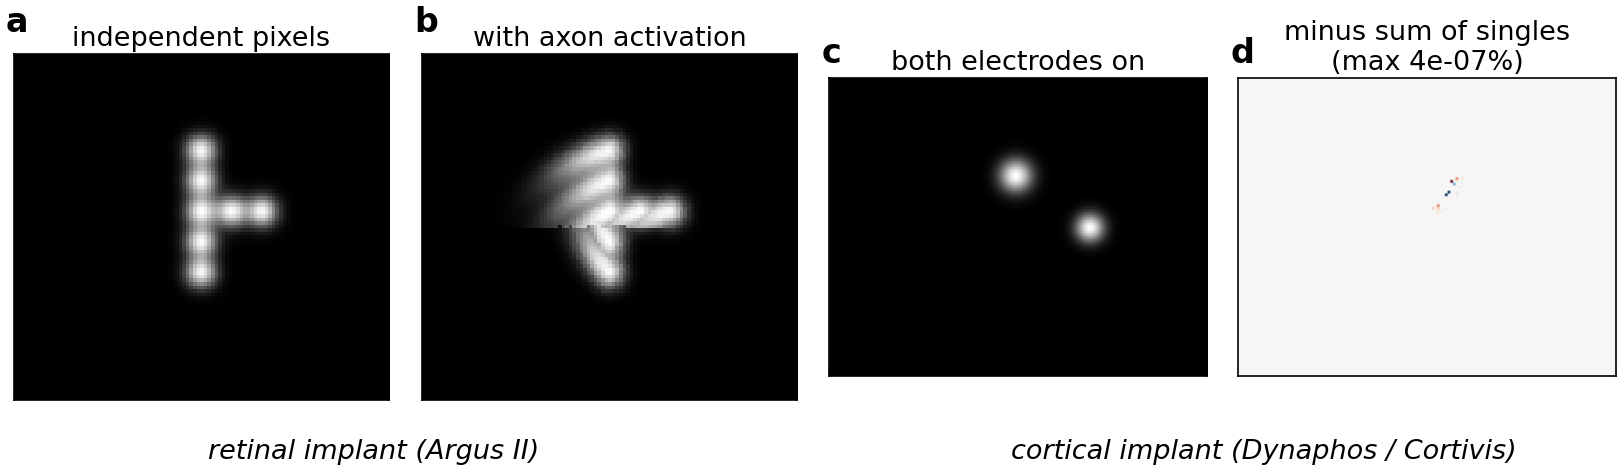
\includegraphics[width=\textwidth]{figures/fig1.png}
\caption{\textbf{The independence assumption and the precedent for doubting
it.} (a) A seven-electrode pattern on an Argus~II retinal implant rendered
by a scoreboard model, in which each electrode is an independent round
phosphene. (b) The same electrodes under an axon-map model that includes
activation of passing ganglion-cell axon bundles. The pattern is no longer
legible. (c) Two Cortivis electrodes driven together at 200~\uA{} under the
Dynaphos cortical baseline. (d) The difference between (c) and the sum of
the two electrodes driven separately, $3.7\times10^{-9}$ of the peak.
That is floating-point noise. Superposition holds exactly in the cortical
baseline by construction.}
\label{fig:f1}
\end{figure}

\begin{figure}[h!]
\centering
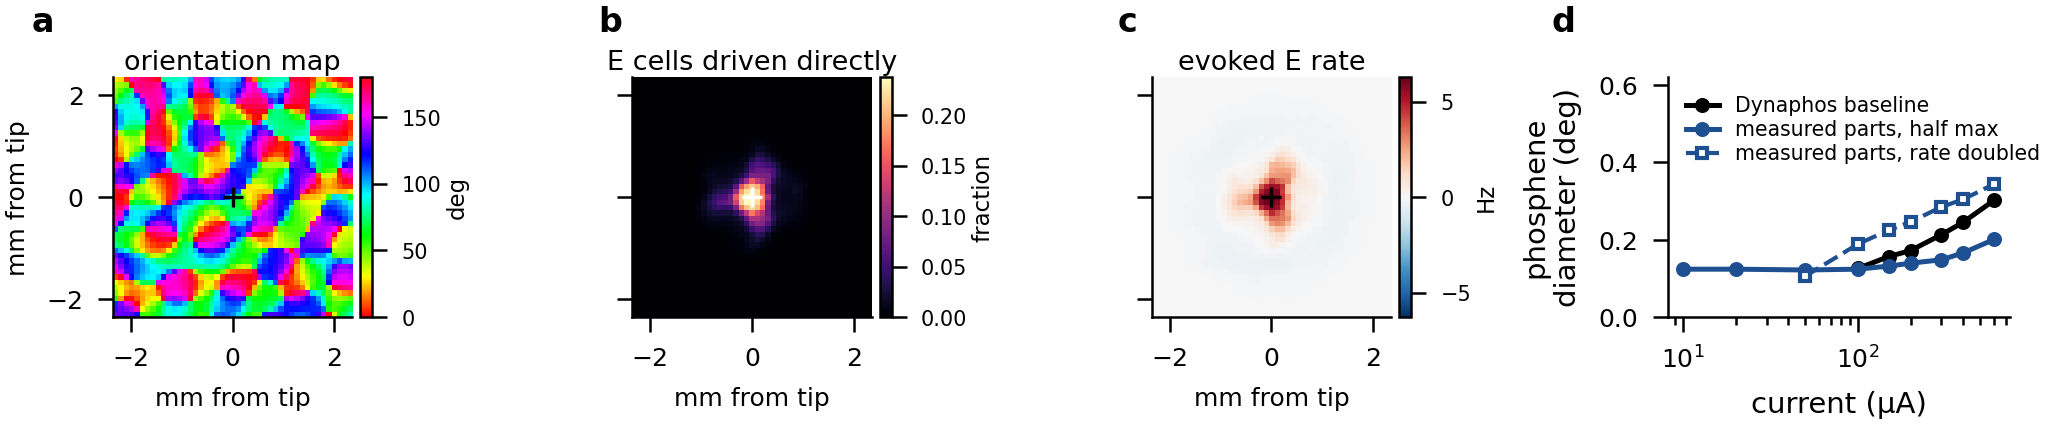
\includegraphics[width=\textwidth]{figures/fig2.png}
\caption{\textbf{The model built from measured parts, and the phosphene it
produces.} (a) Orientation preference map of the simulated sheet, with a
period of 1~mm. (b) Probability that an excitatory cell is directly
recruited by one electrode at 100~\uA. Recruitment is sparse and fills a
region a few hundred microns across. (c) Evoked excitatory rate across the
sheet for the same stimulation, the change from spontaneous activity.
Directly driven cells raise it near the tip, and the network suppresses
ongoing firing around them. (d) Phosphene diameter against current, read
out through the implant's retinotopy, for the Dynaphos baseline (black)
and the model, measured at half maximum (solid) and where firing at least
doubles (dashed). Neither model curve was fitted.}
\label{fig:f2}
\end{figure}

\begin{figure}[h!]
\centering
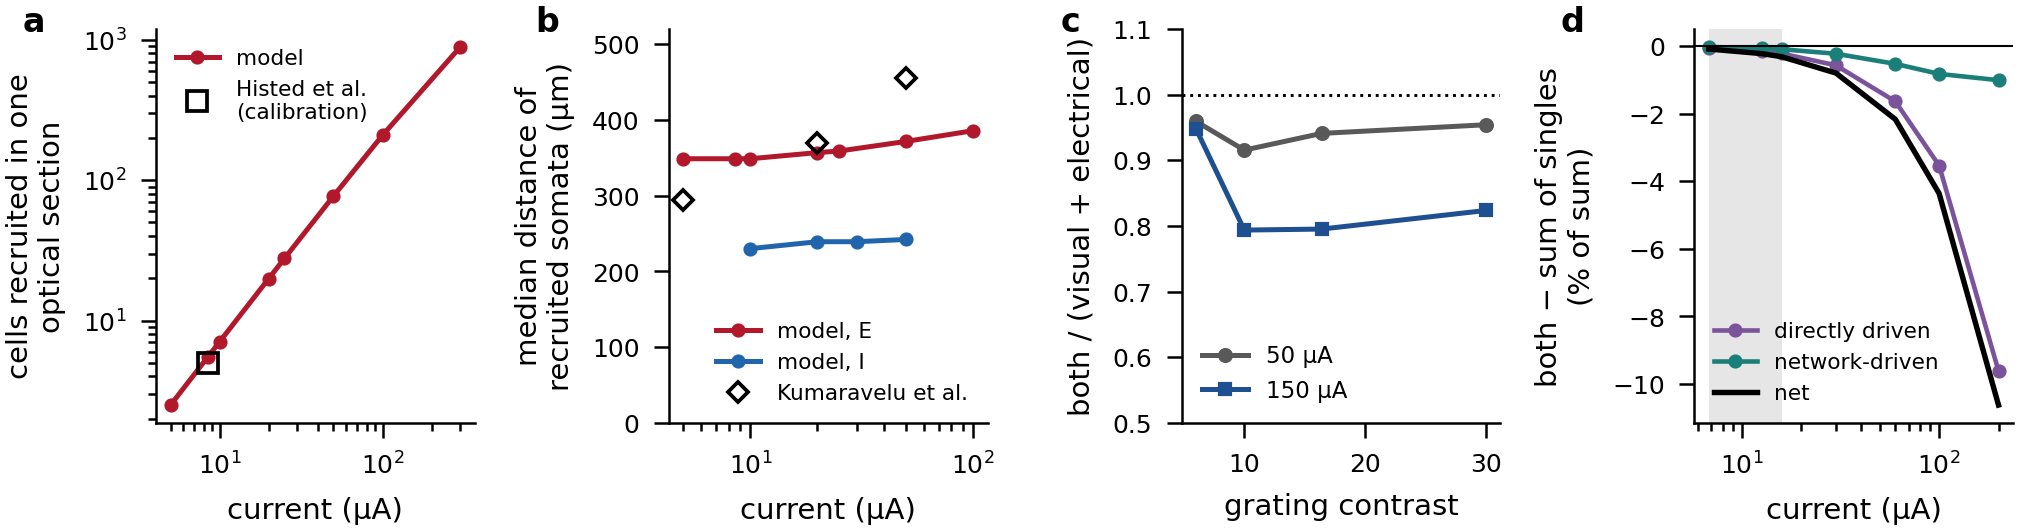
\includegraphics[width=\textwidth]{figures/fig3.png}
\caption{\textbf{The model against measurements.} (a) Cells recruited in
one two-photon optical section against current. The square is the single
calibration point \citep{histed2009}. (b) Median lateral distance of
recruited somata from the tip, for excitatory (red) and inhibitory (blue)
cells. Recruitment fills in with current instead of spreading, and
inhibitory cells are recruited nearer the tip, which the raw cells of
\citet{dadarlat2024} do not show.
Diamonds are the three-dimensional medians of \citet{kumaravelu2022},
which grow faster than the model's. (c) Response at the electrode's own
site to a grating and stimulation together, as a fraction of the two
alone. Summation is sub-additive at every contrast, as \citet{nassi2015}
found. (d) Paired electrodes 485~\um{} apart at 200~Hz, the spacing
\citet{kim2025} used in their own model. The paired response minus the
sum of the single responses, in percent of that sum, over an
$800\times800$~\um{} field between the electrodes. Directly driven cells (purple) are attenuated by
occupancy, and network-driven cells (green) are slightly suppressed.
Shading marks the currents they used. They report net enhancement at the
middle one, which the model does not reproduce.}
\label{fig:f3}
\end{figure}

\begin{figure}[h!]
\centering
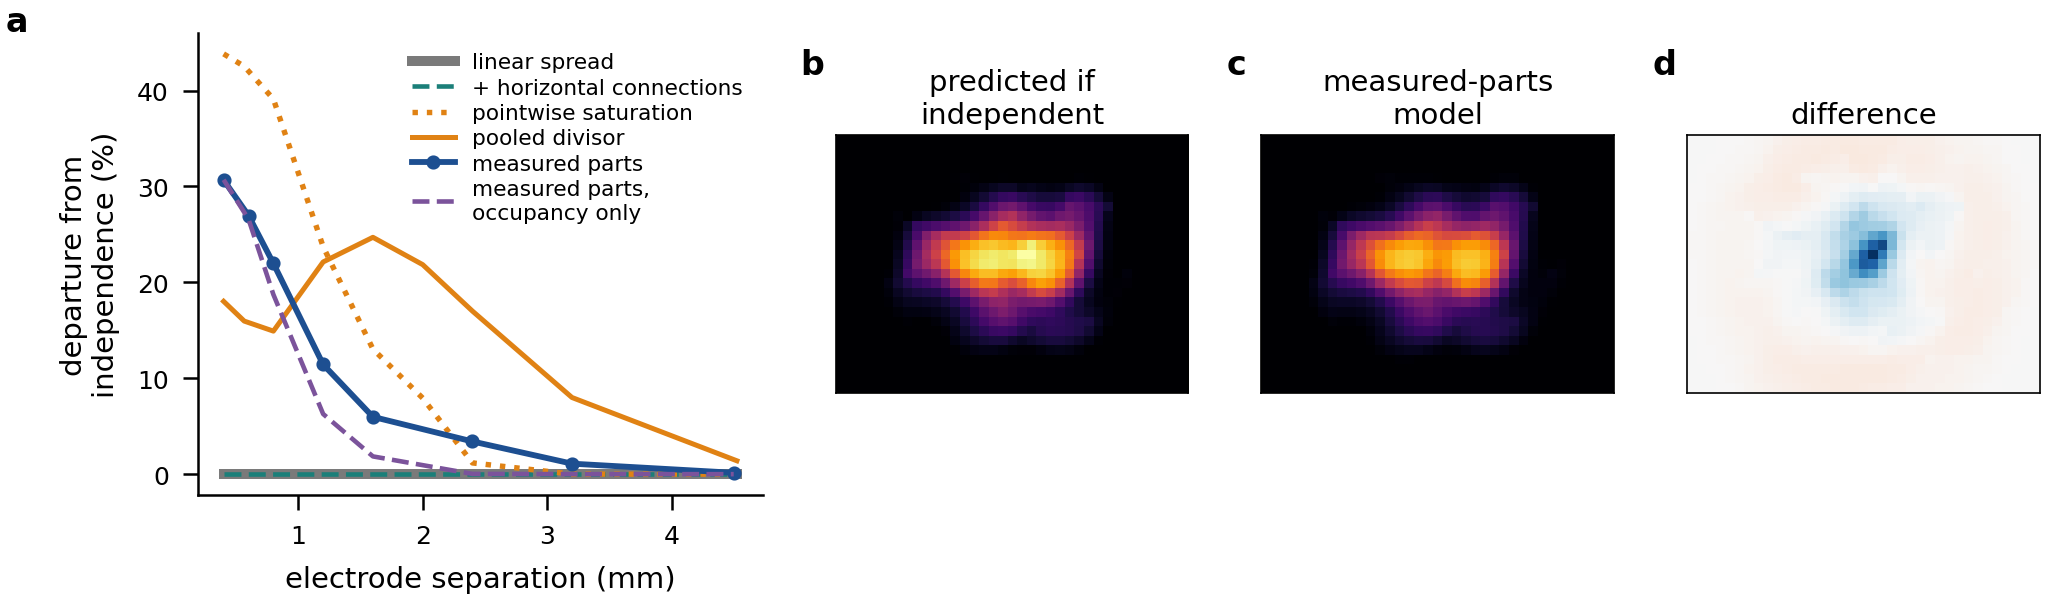
\includegraphics[width=\textwidth]{figures/fig4.png}
\caption{\textbf{Only a nonlinearity acting after the electrodes combine
breaks independence.} (a) Peak departure from linear superposition against
electrode separation, 300~\uA{} per electrode. Linear current spread and
orientation-selective horizontal spread lie on zero. The model built from
measured parts (blue) departs by 31\% at 0.4~mm and decays monotonically,
and its occupancy share alone (purple, dashed) accounts for nearly all of
it. The pooled divisor (orange) peaks in the interior at 1.6~mm, and
pointwise saturation (orange, dotted) is largest at the shortest
separation. (b)--(d) Evoked excitatory rate for two electrodes 0.8~mm
apart at 300~\uA{} in the measured-parts model. The sum of the electrodes
driven alone (b), both driven together (c), and their difference (d) on
its own colour scale. The pair falls short of the sum between the
electrodes, where the same cells are reached twice.}
\label{fig:f4}
\end{figure}

\begin{figure}[h!]
\centering
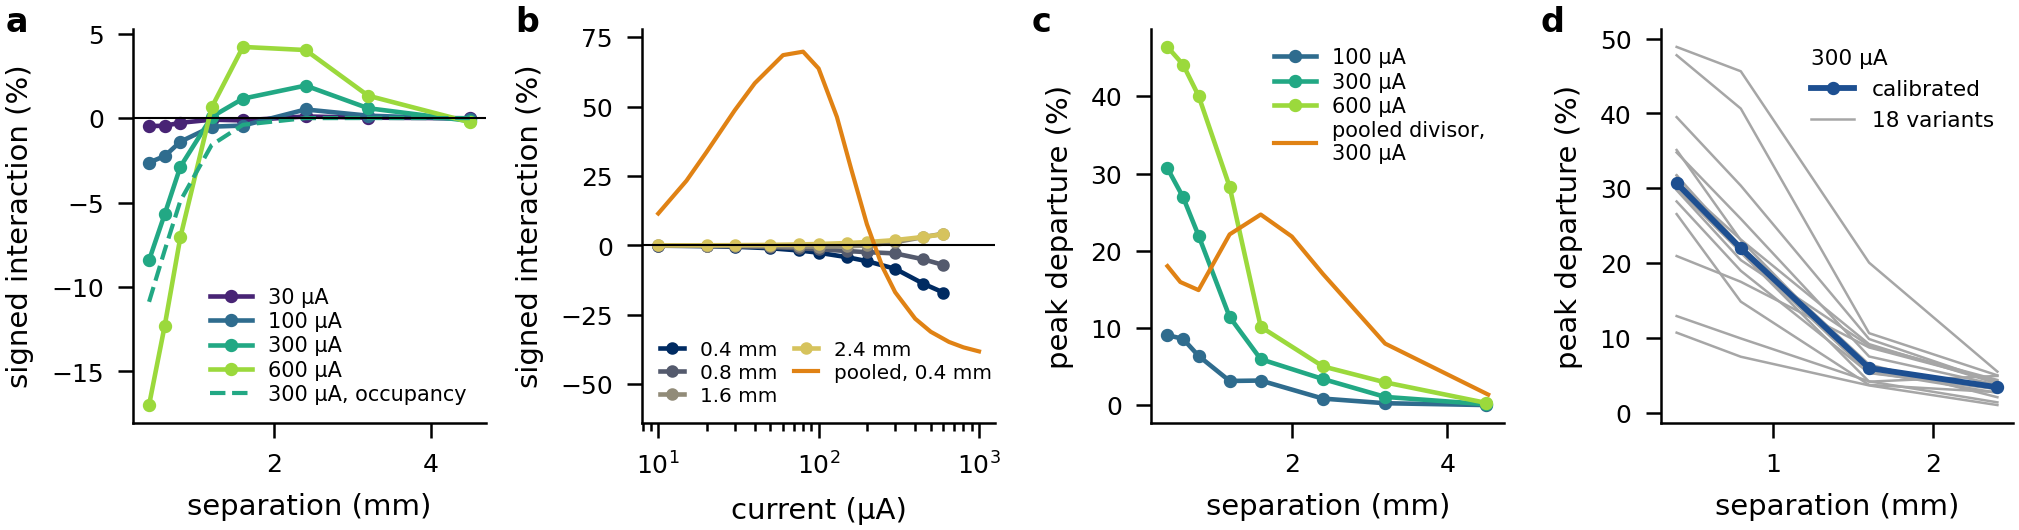
\includegraphics[width=\textwidth]{figures/fig5.png}
\caption{\textbf{Magnitude, shape and sign in the model built from
measured parts.} (a) Signed interaction, summed over the sheet, against
separation at four currents. It is suppressive at short range at every
current and slightly facilitatory at intermediate range. The dashed line is
the occupancy share at 300~\uA, which accounts for most of it. (b) The same
quantity against current at four separations. At 0.4 and 0.8~mm it is
suppressive at every current, and the pooled divisor at 0.4~mm (orange)
crosses from facilitation to suppression. (c) Peak departure against
separation. It is largest at the shortest separation and decays
monotonically, the pointwise shape, while the pooled divisor peaks in the
interior. (d) Peak departure at 300~\uA{} for the calibrated model and
the eighteen variants of table~\ref{tab:t4}. Every variant peaks at the
shortest separation.}
\label{fig:f5}
\end{figure}

\begin{figure}[h!]
\centering
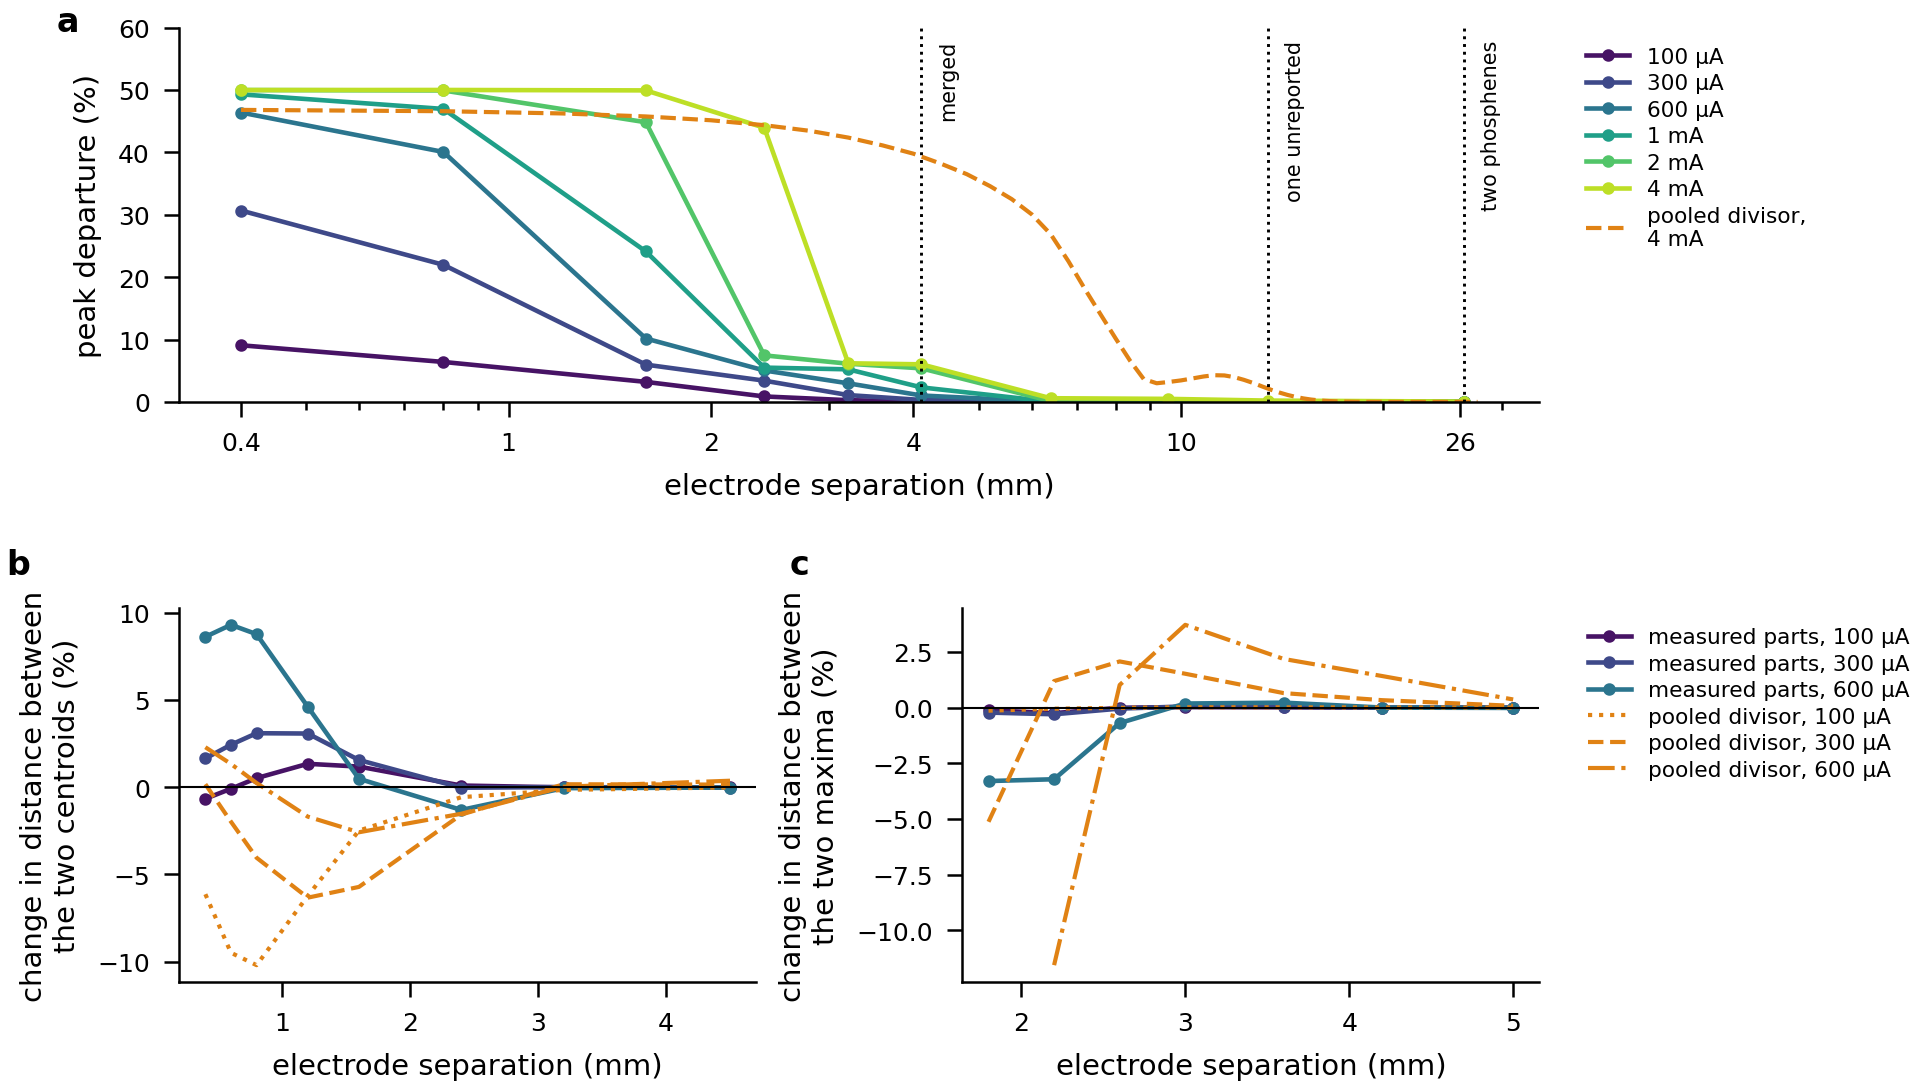
\includegraphics[width=\textwidth]{figures/fig6.png}
\caption{\textbf{The human multi-electrode data.} (a) Peak departure from
superposition against separation, on a logarithmic axis, from 100~\uA{}
to 4~mA. Dotted lines mark the mean separations reported by
\citet{bosking2022} for pairs that merged, pairs in which one phosphene
went unreported, and pairs seen as two phosphenes. Above 0.6~mA the model
extrapolates recruitment far past its calibration. The dashed orange line
is the pooled divisor at 4~mA. (b) Change in the distance between the two
activity centroids when the electrodes are driven together, relative to
the sum of the electrodes driven alone. Positive values mean the two
regions of activity push apart. The estimator gives exactly zero for any
linear model. (c) The same for the distance between the two maxima along
the line joining the electrodes, from 1.8~mm, where the two maxima are
still separate. In (b) and (c) the pooled divisor (orange) is measured
with the same estimator at the same currents.}
\label{fig:f6}
\end{figure}

\begin{figure}[h!]
\centering
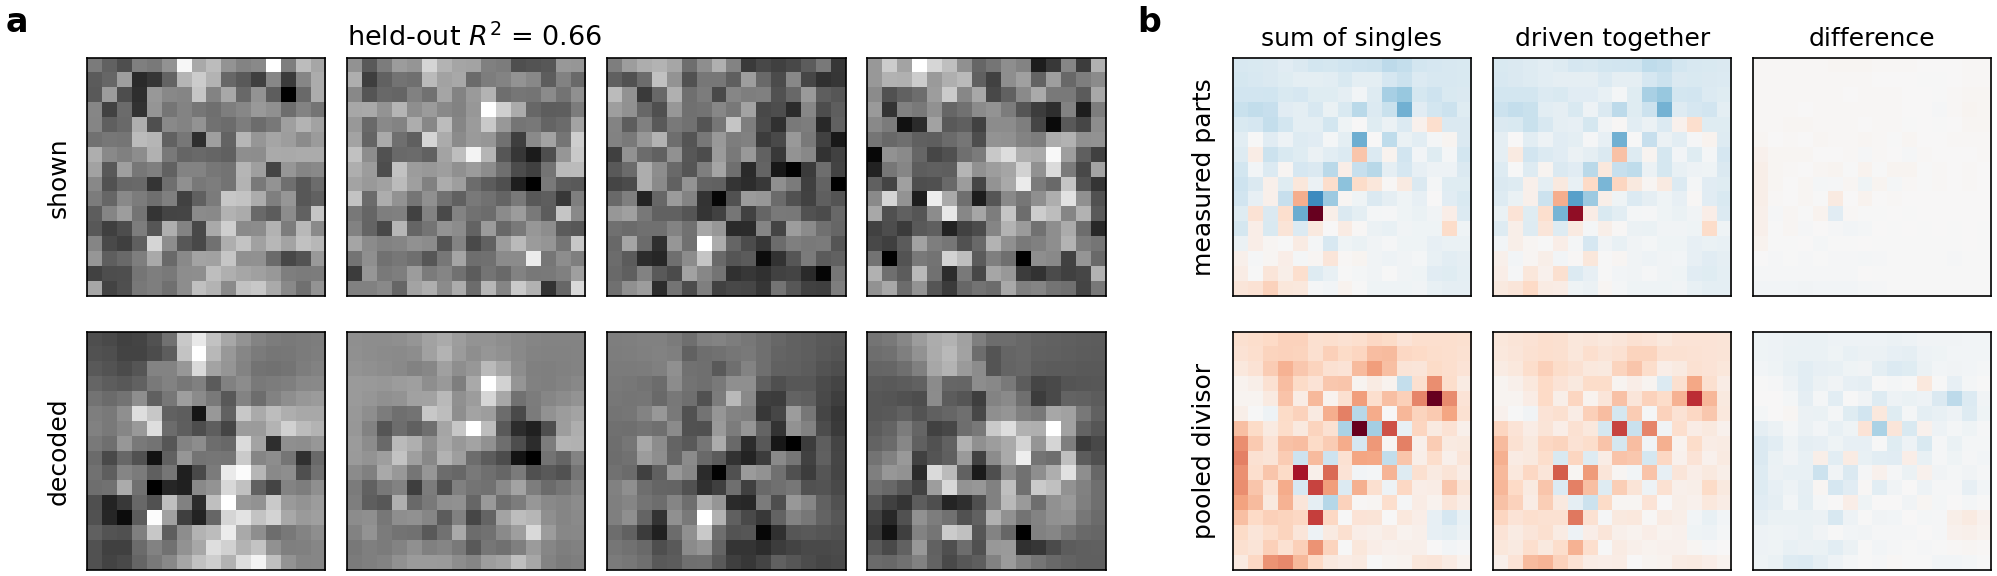
\includegraphics[width=\textwidth]{figures/fig7.png}
\caption{\textbf{Percepts.} (a) Held-out validation of the decoder on the
measured-parts model's orientation map. $1/f$ noise images shown to the
model's visual pathway (top) and recovered from the resulting cortical
activity (bottom), $R^2 = 0.66$ over 24 held-out images of which four are
shown. (b) Five electrodes, 0.9 to 1.8~mm from their nearest neighbours,
at 300~\uA. The sum of
the percepts of each electrode driven alone, the percept of all five
driven together, and their difference, for the model built from measured
parts (top) and the pooled divisor (bottom), each decoded through its own
model's map with the same linear operator and shown on one colour scale
per row.}
\label{fig:f7}
\end{figure}

\begin{figure}[h!]
\centering
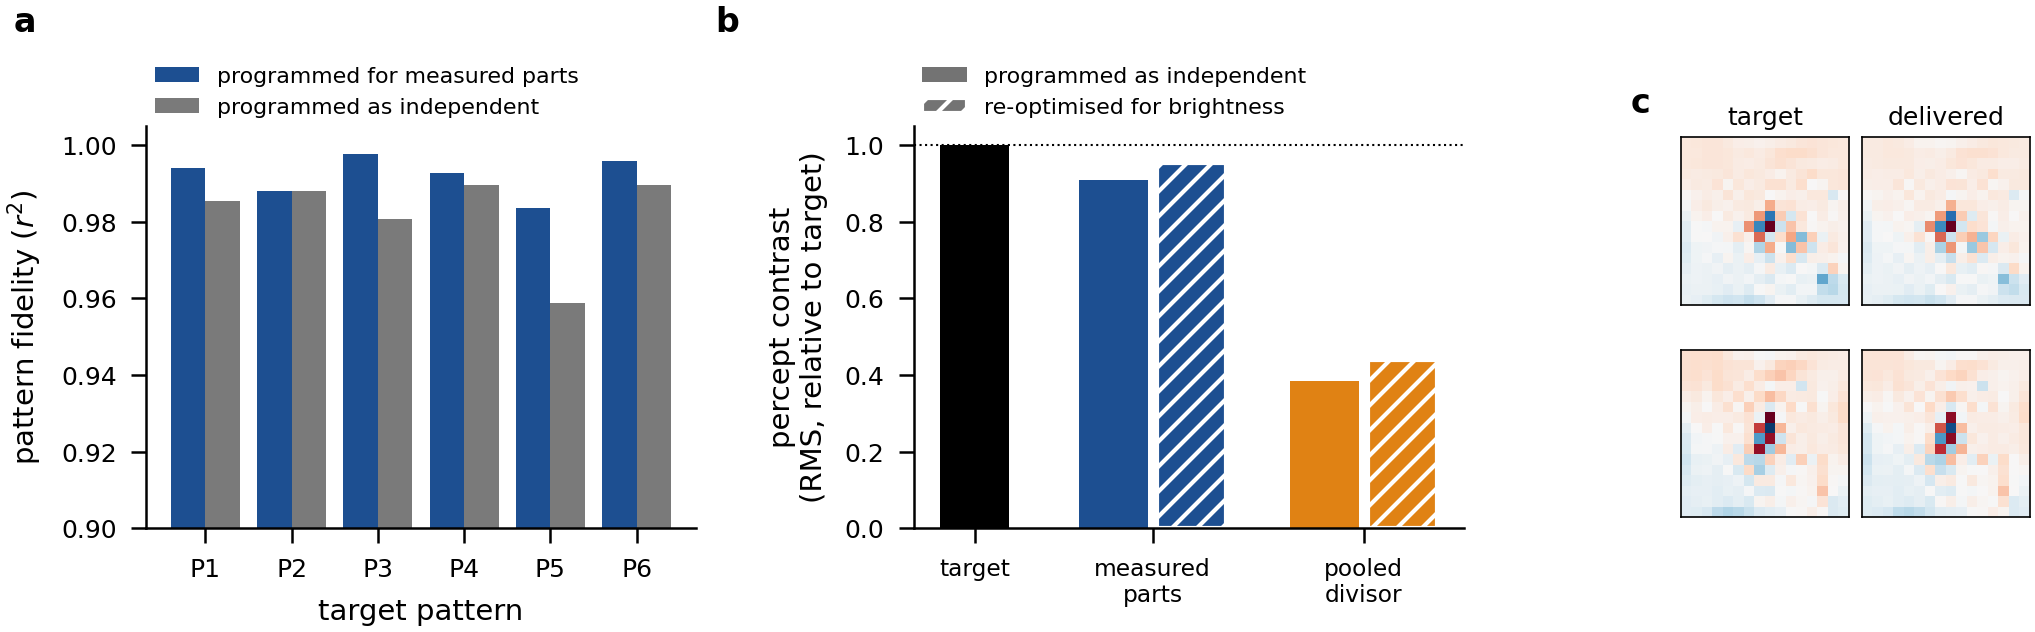
\includegraphics[width=\textwidth]{figures/fig8.png}
\caption{\textbf{Stimulation programmed as though electrodes were
independent.} (a) Pattern fidelity for six deliverable targets in the
model built from measured parts, for stimulation optimised under the full
model and for stimulation optimised under independence, both delivered to
the full model. (b) Percept contrast relative to the target. Programmed as
independent and delivered (solid), and after re-optimising an objective
that seeks brightness (hatched), for the model built from measured parts
(blue) and the pooled divisor (orange). (c) Two of the targets and what
the measured-parts model delivers when they are programmed under
independence.}
\label{fig:f8}
\end{figure}

\begin{figure}[h!]
\centering
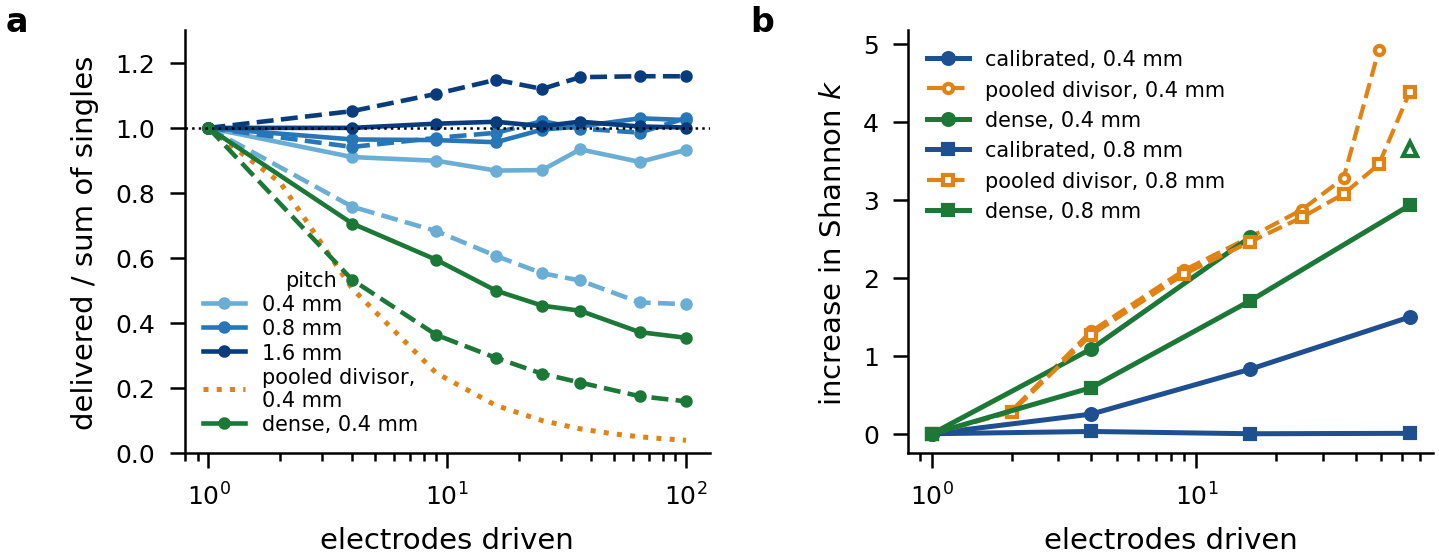
\includegraphics[width=\textwidth]{figures/fig9.png}
\caption{\textbf{Arrays.} (a) Output of $N$ electrodes driven together
relative to the sum of the same electrodes driven alone, in the model
built from measured parts at three pitches, at 100~\uA{} (solid) and
300~\uA{} (dashed). The ratio levels off without falling as $1/N$. The
pooled divisor at 400~\um{} pitch (orange, dotted) falls toward its
ceiling. (b) Increase in Shannon's $k = \log_{10}D + \log_{10}Q$ needed to
hold per-channel output at its single-electrode value from a 300~\uA{}
reference. Because charge and charge density both scale with amplitude,
the increase does not depend on electrode area or pulse width. Curves stop
where the required amplitude exceeds 200~mA.}
\label{fig:f9}
\end{figure}

\begin{figure}[h!]
\centering
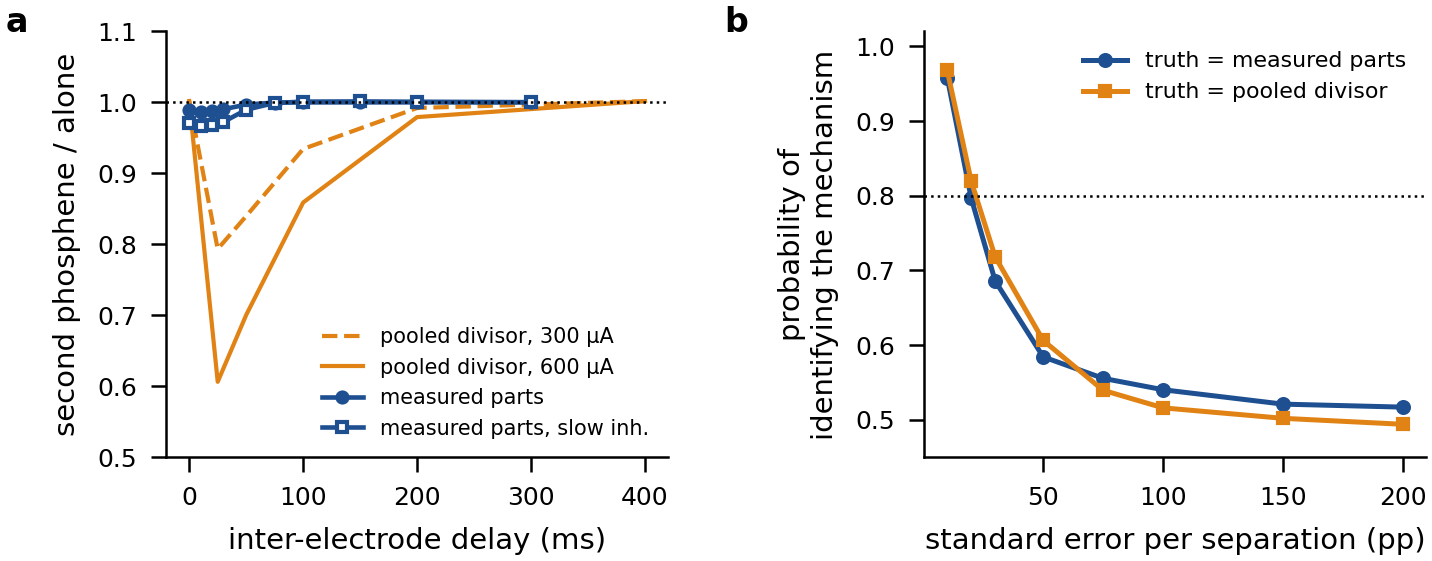
\includegraphics[width=0.72\textwidth]{figures/fig10.png}
\caption{\textbf{Sequences, and what it costs to tell the hypotheses
apart.} (a) Brightness of the second of two phosphenes 1.6~mm apart,
relative to the same electrode alone, against delay. The model built from
measured parts at 300~\uA, with fast inhibition only (filled) or 30\% slow
inhibition (open), stays within a few percent of one. The pooled divisor
(orange) makes the later phosphene dimmer, which two of the three subjects
in \citet{armentasalas2022} contradict. (b) Probability of identifying the
true hypothesis from the shape of interaction against separation, with a
scale-free decision rule, against the standard error per separation.}
\label{fig:f10}
\end{figure}

\begin{figure}[h!]
\centering
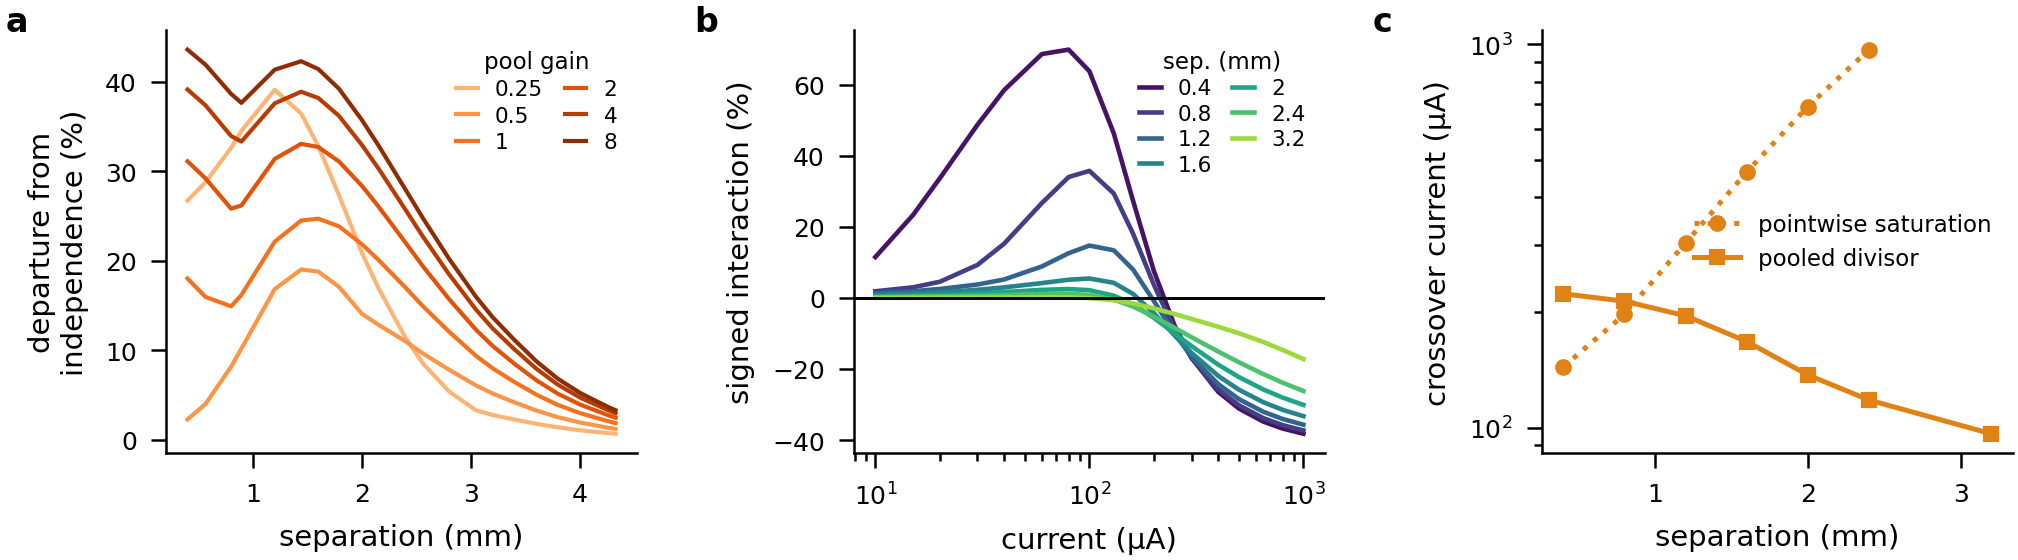
\includegraphics[width=\textwidth]{figures/fig11.png}
\caption{\textbf{The pooled divisor.} (a) Peak departure against
separation for normalisation gains spanning 32-fold, with $K$ refitted at
every point so that all of them reproduce the single-electrode curve. The
magnitude changes about two-fold and the interior peak does not move. (b)
Signed interaction against current for the full pooled-divisor model, one
curve per separation, positive being facilitation. Every separation
crosses from facilitation to suppression. (c) The current at which the
sign flips, against separation. It falls for the pooled divisor and rises
for pointwise saturation, whose interaction lives only in the overlap.}
\label{fig:f11}
\end{figure}

\begin{figure}[h!]
\centering
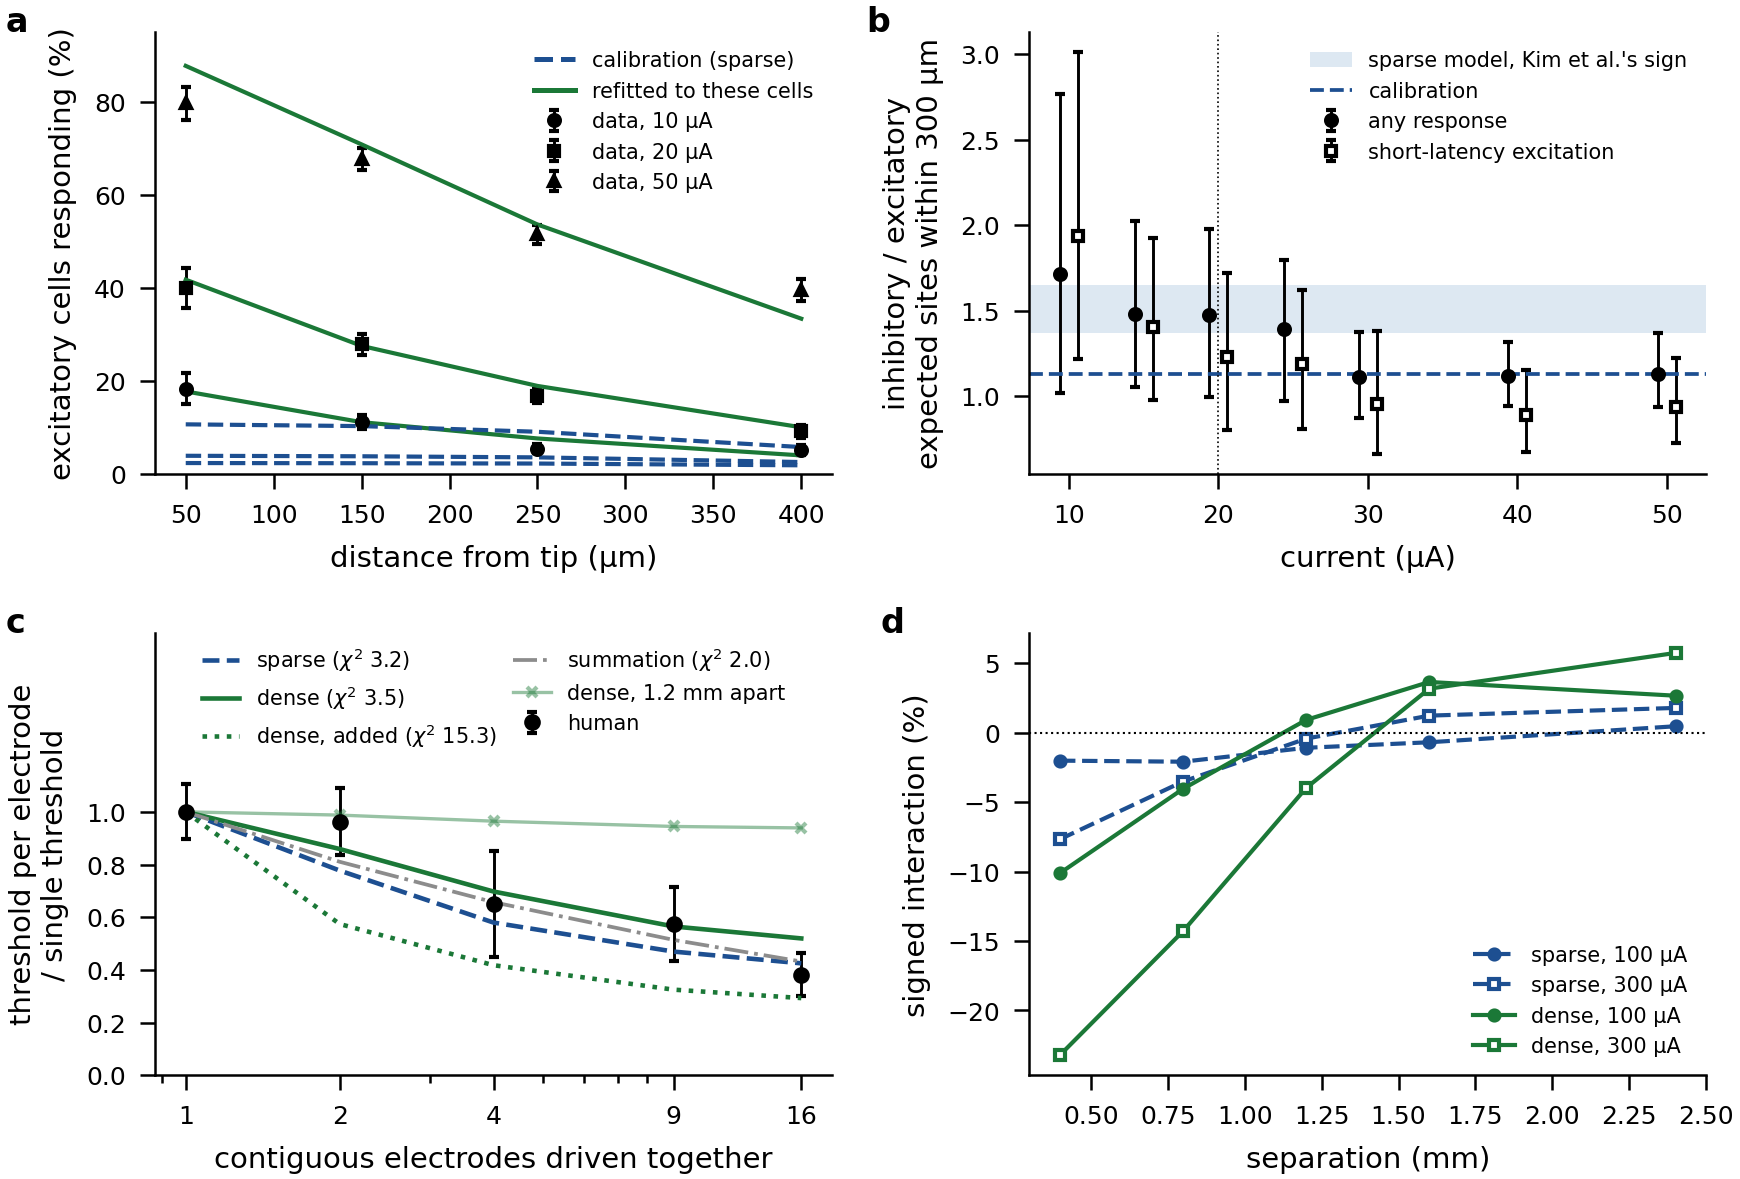
\includegraphics[width=\textwidth]{figures/fig12.png}
\caption{\textbf{The model against raw cells from awake cortex and against
human thresholds.} (a) Excitatory cells responding to one electrode in
awake mouse V1 \citep{dadarlat2023data}, against distance from the tip, at
10, 20 and 50~\uA{} (points, with binomial 95\% intervals). The calibrated
recruitment (blue, dashed) predicts a tenth of the responses at every
distance. Recruitment refitted to these cells, with a local core of
88~\um{} (green), follows them. (b) Inhibitory to excitatory ratio of
expected sites within 300~\um, read from the raw cells with saturation
undone, for any response (filled) and short-latency excitation (open),
with hierarchical-bootstrap 95\% intervals. The band is the range the
sparse model needs for the sign of Kim \textit{et al.}'s net modulation,
and the dashed line the calibration. (c) Per-electrode threshold for groups
of contiguous Utah electrodes at 400~\um{} pitch in a blind volunteer
\citep{fernandez2021}, relative to one electrode, against the model with a
local readout ($\sigma=100$~\um) and the single threshold at 73.5~\uA.
Sparse and dense recruitment with occupancy both fit. Dense recruitment
with activations added where they overlap does not. Probability summation
over independent electrodes (grey) fits as well. The pale line is the
model's prediction for the same groups on every third electrode, 1.2~mm
apart, where probability summation predicts the grey curve again. (d) Signed interaction
against separation with calibrated (dashed) and dense (solid) recruitment,
at 100 and 300~\uA{} on a 53.5~\um{} grid.}
\label{fig:f12}
\end{figure}

\end{document}
